\documentclass[11pt]{article}

% Encoding
\usepackage[utf8]{inputenc}
\usepackage[T1]{fontenc}

% Professional preprint style (shared with the Latent Bridge paper):
% Palatino body + matching math, Helvetica-clone sans headings, ruled header.
% arxiv.sty already provides xcolor, microtype, and caption.
\usepackage{arxiv}

% Content packages
\usepackage{amsmath}
\usepackage{amssymb}
\usepackage{amsfonts}
\usepackage{graphicx}
\usepackage{float}
\usepackage{booktabs}
\usepackage{subcaption}
\usepackage{multirow}
\usepackage{array}
\usepackage{nicefrac}
\usepackage{tcolorbox}

% hyperref loaded late, then coloured to match the palette.
\usepackage{hyperref}
\usepackage{url}
\hypersetup{
  colorlinks=true,
  linkcolor=arxivaccent,
  citecolor=arxivaccent,
  urlcolor=arxivaccent,
  filecolor=arxivaccent,
  breaklinks=true,
}

% Tolerate slightly looser lines rather than overflow the margin on
% paragraphs with long verbatim file paths and tightly-packed tables.
\emergencystretch=3em

% Box style for the running example (verbatim artifacts from the released runs).
\newtcolorbox{examplebox}{colback=arxivaccent!4!white,colframe=arxivaccent!60!black,
  boxrule=0.5pt,arc=2pt,left=6pt,right=6pt,top=5pt,bottom=5pt}

\title{Transcribe, Then Reason:\\
Two-Pass Decomposition for Multimodal Review}

\author{%
  \begin{tabular}{@{}c@{\hspace{4em}}c@{}}
    Bojie Li & Noah Shi \\
    Pine AI & University of Washington
  \end{tabular}%
}
\date{}
\runningtitle{Transcribe, Then Reason: Two-Pass Decomposition for Multimodal Review}

\begin{document}

\maketitle
\vspace{-1.2em}

% =================================================================
\begin{abstract}
The default approach to long-form multimodal review is end-to-end: give a model raw audio or page images and ask it to write the review in one call. Across 21 review cells, this approach quietly \emph{satisfices}: it drops roughly a third of the source content and embellishes what remains. This is not primarily a perception failure: $99.7\%$ of the dropped content appears in the same model's transcript of the same source. Our nine-experiment mechanistic study instead identifies \textbf{generation under load} as the bottleneck. For legible propositional content, models read text and images of the same text equally well; the difficulty is asking one pass to perceive, reason, and write a long, faithful review simultaneously. The resulting intervention is simple: use two same-weights passes, first to transcribe and then to review the transcript, with a full output budget for each. This decomposition improves faithfulness in 18/21 cells and coverage in 16/21; both effects are sign-test significant and stable under $n{=}5$ reruns. Its gain scales inversely with end-to-end performance ($r{=}-0.45$): the more the monolithic pass satisfices, the more decomposition recovers. The same headroom law organizes the cross-vendor and mixed-model results, where decomposition also lets text-only frontier models review audio. It further predicts two observed failure modes: synthesis-budget overflow on very long sources and training-prior confabulation after the grounding modality is removed. The benefit is the decomposition, not the modality.
\end{abstract}
\vspace{-0.4em}
\begin{center}
\footnotesize
Code: \url{https://github.com/19PINE-AI/cascade-gap} \quad$\cdot$\quad Website: \url{https://01.me/research/cascade-gap}
\end{center}
\vspace{-1.2em}

\begin{figure}[H]
\centering
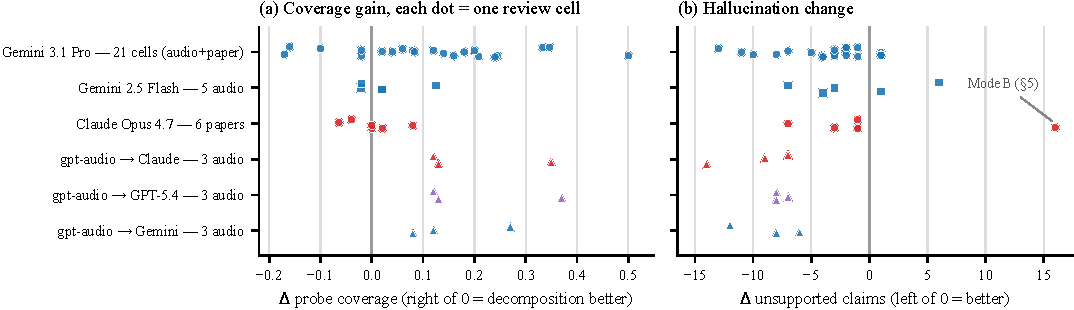
\includegraphics[width=\linewidth]{figures/fig1_showcase.pdf}
\vspace{-8pt}
\caption{\textbf{Two-pass decomposition improves long-form review.} Each dot is one cell's change from end-to-end ($C_0$) to transcribe-then-review ($C_1$): \textbf{(a)} probe coverage and \textbf{(b)} unsupported claims. Rows use the same weights; \texttt{gpt-audio} rows are mixed pipelines. Coverage improves on 16/21 cells and unsupported claims fall on 18/21 (sign tests $p{=}0.027$, $p{=}0.0015$).}
\label{fig:headline}
\end{figure}

% =================================================================
\section{Introduction}
\label{sec:intro}

\begin{figure}[t]
\centering
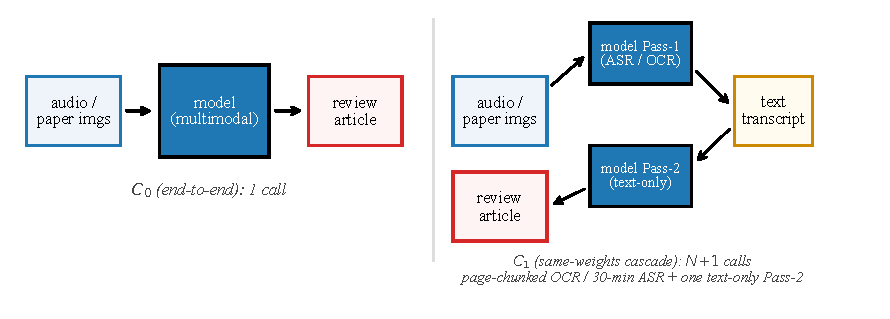
\includegraphics[width=0.72\linewidth]{figures/fig0_protocol_schematic.pdf}
\caption{\textbf{Two configurations with the same weights.} $C_0$ writes from raw audio or page images in one call. $C_1$ transcribes first, then writes from that transcript alone; only the reasoning step's input representation differs.}
\label{fig:schematic}
\end{figure}

Multimodal foundation models can read audio and document images directly. It is therefore natural to use them end-to-end for long-form review: provide the raw source and request a review in one call (Figure~\ref{fig:schematic}, top). Keeping the original modality in context seems strictly safer: transcription can lose information, whereas the model can see or hear the entire source.

This paper tests that intuition for long-form review and finds the opposite result.

\textbf{The observation (\S\ref{sec:observation}).} Frontier models quietly satisfice when they review long sources end-to-end. In our running example---Andrej Karpathy's 42-minute \emph{State of GPT} talk---Gemini~3.1~Pro's review covers only about six in ten atomic facts extracted by an independent judge, and about one quarter of its claims are unsupported (Figure~\ref{fig:example}). This is not a perception failure. When prompted only to transcribe the same audio, the same model produces a transcript containing every fact its review omitted. Across all 21 cells, $99.7\%$ of content omitted by the end-to-end pass appears in the model's own transcript (Figure~\ref{fig:mech_e3}); in the running example, the omitted sentences appear verbatim. The content is perceived but lost downstream.

\textbf{The mechanism (\S\ref{sec:mechanism}).} Three explanations fit this observation. The \emph{modality hypothesis} holds that models reason better over text than over raw audio or pixels. The \emph{generation-load hypothesis} holds that a single pass cannot simultaneously perceive, reason over, and write a long faithful review. The \emph{attention-dilution hypothesis} holds that long sequences of low-density modality tokens dilute attention. Nine experiments distinguish these accounts. The modality hypothesis fails in every setting we can test: models read identical propositional content equally well from text and from an \emph{image} of that text, both in open-VLM activations and behaviorally on the frontier models. Under reasoning load, images are, if anything, better (Figure~\ref{fig:substrate}). Generation load does bind: asking one call to transcribe and review sharply reduces coverage or produces no review, whereas giving a transcript-equipped pass access to the raw modality changes little (Figure~\ref{fig:e2_collapse}). The bottleneck is the single pass, not the pixels.

\textbf{The solution (\S\ref{sec:solution}).} The mechanism suggests giving each step a dedicated, full-budget pass. Pass~1 transcribes the source (\emph{perceive and externalize}); Pass~2 writes the review from that transcript alone (\emph{synthesize}), using the same weights throughout. This two-pass decomposition ($C_1$) outperforms end-to-end review ($C_0$) on faithfulness and coverage across the 21-cell suite (Figure~\ref{fig:headline}). Its gain follows an \emph{inverse-baseline law}: it grows with the extent to which the monolithic pass satisfices ($r{=}-0.45$, Figure~\ref{fig:solution}). This is not a uniform improvement, but the same law organizes the cross-vendor results (Figure~\ref{fig:xmodel}) and predicts two observed failure modes: synthesis-budget overflow on very long sources (Mode~A), and training-prior confabulation after the grounding modality is removed (Mode~B). We test a quote-grounded refinement for the latter (\S\ref{sec:failure_modes}).

\paragraph{Contributions.}
(1)~A 21-cell, same-weights comparison of end-to-end and two-pass long-form review across two modalities, three vendors, and two judges (\S\ref{sec:observation}, \S\ref{sec:solution}).
(2)~A nine-experiment mechanism study that distinguishes perception, modality, and generation-side accounts. It rules out the first two in the tested regime---including through behavioral probes on the frontier models---and supports \textbf{perceive--externalize--synthesize} (\S\ref{sec:mechanism}).
(3)~A two-mode account of when decomposition fails, with mechanism-derived deployment triggers, two tested interventions, and a quote-grounded iterative-refinement variant (\S\ref{sec:failure_modes}).
(4)~Robustness checks comprising inter-judge replication on all 21 cells, probe re-extraction, reference regeneration, and $n{=}5$ multi-seed verification; we report every preserved and retracted result (\S\ref{sec:robust}).

% =================================================================
\section{The observation: end-to-end long-form review satisfices}
\label{sec:observation}

\begin{figure}[!t]
\begin{examplebox}
\small
\textbf{Running example: Gemini 3.1 Pro reviews Karpathy's \emph{State of GPT} (42-min audio), end-to-end.}
All excerpts are verbatim from the released run artifacts.\\[4pt]
\textbf{The talk says:} \emph{``The vocabulary size is usually a couple ten thousand tokens''} --- and the model hears it: its own transcript of the audio contains the sentence verbatim.\\[2pt]
\textbf{The end-to-end review writes:} \emph{``A typical vocabulary size is around 10{,}000 tokens.''} --- one of \textbf{13 unsupported claims}, alongside a misdescription of RLHF as a fourth serial pipeline stage.\\[4pt]
\textbf{The talk ends with} Karpathy prompting GPT-4: \emph{``can you say something to inspire the audience of Microsoft Build 2023?''} --- again present verbatim in the model's own transcript.\\[2pt]
\textbf{The end-to-end review:} drops it entirely, one of \textbf{19 of 51 probes missed}. All 19 missed probes are present in the model's own 8{,}500-word transcript of the same audio.\\[4pt]
\textbf{The two-pass review} (\S\ref{sec:solution}: same weights, written from that transcript alone) covers \textbf{49 of 51 probes with 3 unsupported claims}, and gets the example right: \emph{``Vocabulary sizes are usually a couple ten thousand tokens (e.g., 50{,}257).''}
\end{examplebox}
\vspace{-2pt}
\caption{\textbf{Running example.} The end-to-end review drops perceived content and adds unsupported detail; the two-pass review recovers coverage and faithfulness. Karpathy is the bolded row in Figure~\ref{fig:headline_cells}a.}
\label{fig:example}
\end{figure}

\paragraph{Task and protocol.}
Our task is long-form review: given a 26--85-minute recording or a 9--176-page paper supplied as page images, write a review that is \emph{exhaustive} (covers the source's content) and \emph{faithful} (adds no unsupported content). For each source, Gemini~3.1~Pro produces a chunked ASR/OCR reference transcript (30-minute audio chunks; one page per OCR call; Appendix~\ref{appdx:protocol}). GPT-5.4 (\texttt{reasoning\_effort=high}) then extracts roughly 50 atomic factual probes from the reference (47--51 per cell), scores each review as COVERED or MISSING on each probe, and lists unsupported claims. We treat $|\Delta h|\le 1$ on low-count cells and $|\Delta_{\rm cov}|\le 0.04$ as within noise, and report Wilson and bootstrap CIs and aggregate sign tests (Appendix~\ref{appdx:protocol}). The suite contains 21 Gemini cells: 11 audio cells from 10 recordings (talks, lectures, panels, and meetings) and 10 papers (seven 1968--1972 NASA reports and three post-cutoff 2026 arXiv reviews; Appendix~\ref{appdx:cell_table}). We first evaluate $C_0$, the end-to-end configuration in which the model reads the raw modality and writes the review in one call.


\paragraph{The end-to-end pass drops a third of the content\ldots}
Figure~\ref{fig:headline_cells} (gray points) summarizes $C_0$ across the suite: mean probe coverage is $0.65$, and every cell contains unsupported claims. The running example (Figure~\ref{fig:example}) illustrates the resulting errors: invented precision (``10{,}000 tokens''), a structural misdescription (RLHF as a fourth stage), and omitted content (the talk's closing demonstration).

\paragraph{\ldots that it demonstrably perceived (the perception check).}
A natural explanation is that the model cannot hear or read the source well enough. To test this, we asked the same model to \emph{transcribe} each source using the chunked ASR/OCR procedure that produces the reference, then scored the transcript against the same probes. The transcript covers essentially every probe in every cell (Figure~\ref{fig:mech_e3}), far more than the review written from the same input. Across the suite, $361$ of the $362$ probes omitted by the end-to-end pass ($99.7\%$) appear in the model's own transcript; the corresponding figure for Karpathy is 19 of 19. Because the probes come from a near-identical reference, the transcript ceiling is partly definitional. The key inference is narrower: the content omitted by the end-to-end review \emph{is} capturable as text by the same model. The loss therefore occurs downstream of perception---the puzzle addressed in the next section.

\begin{figure}[t]
\centering
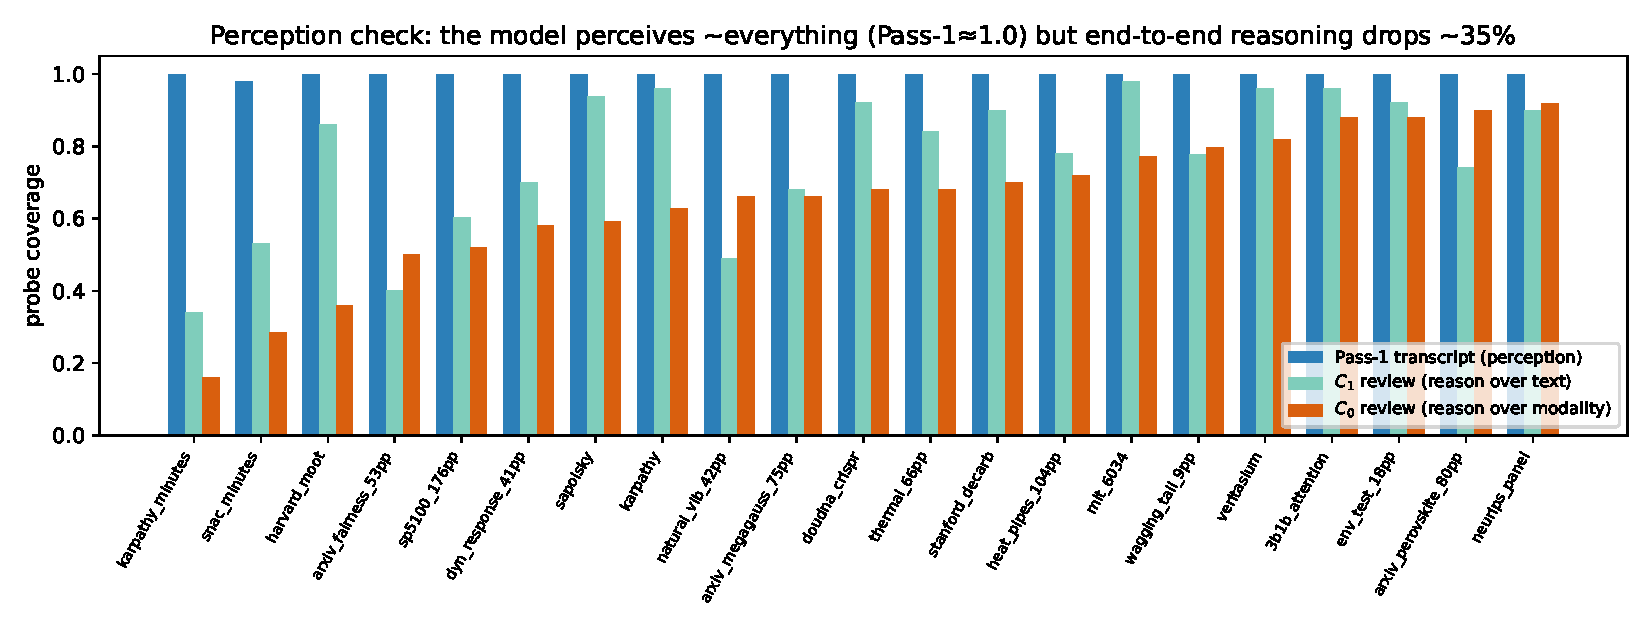
\includegraphics[width=0.9\linewidth]{figures/fig_mech_e3.pdf}
\caption{\textbf{Perception check.} Per cell, the model's transcript (blue) covers nearly all probes, versus mean coverage of $0.65$ for $C_0$ (orange) and $0.77$ for $C_1$ (green). Of the probes $C_0$ drops, $361/362$ ($99.7\%$; Wilson 95\% CI $[98.5\%,99.9\%]$) appear in its transcript.}
\label{fig:mech_e3}
\end{figure}

% =================================================================
\section{Mechanism: why one pass fails}
\label{sec:mechanism}

Three hypotheses explain the observation in \S\ref{sec:observation}, but make different predictions. The \textbf{modality hypothesis} is that models reason better over text than raw audio or image tokens. The \textbf{generation-load hypothesis} is that one pass cannot simultaneously perceive, reason over, and write a long faithful review; each step therefore needs a dedicated output budget. The \textbf{attention-dilution hypothesis} is that long, low-density modality-token sequences dilute attention. We ran nine experiments, using the same probe and hallucination judge throughout (artifacts: \S\ref{appdx:code}). The results reject the modality hypothesis in every test available to us and support the generation-load hypothesis through two load-bearing, multi-seed contrasts across all 21 cells. Our tools cannot test attention dilution on Gemini, because its image pipeline normalizes away DPI differences. Appendix~\ref{appdx:substrate} gives the per-experiment details.

\begin{figure}[t]
\centering
\begin{subfigure}{\linewidth}
\centering
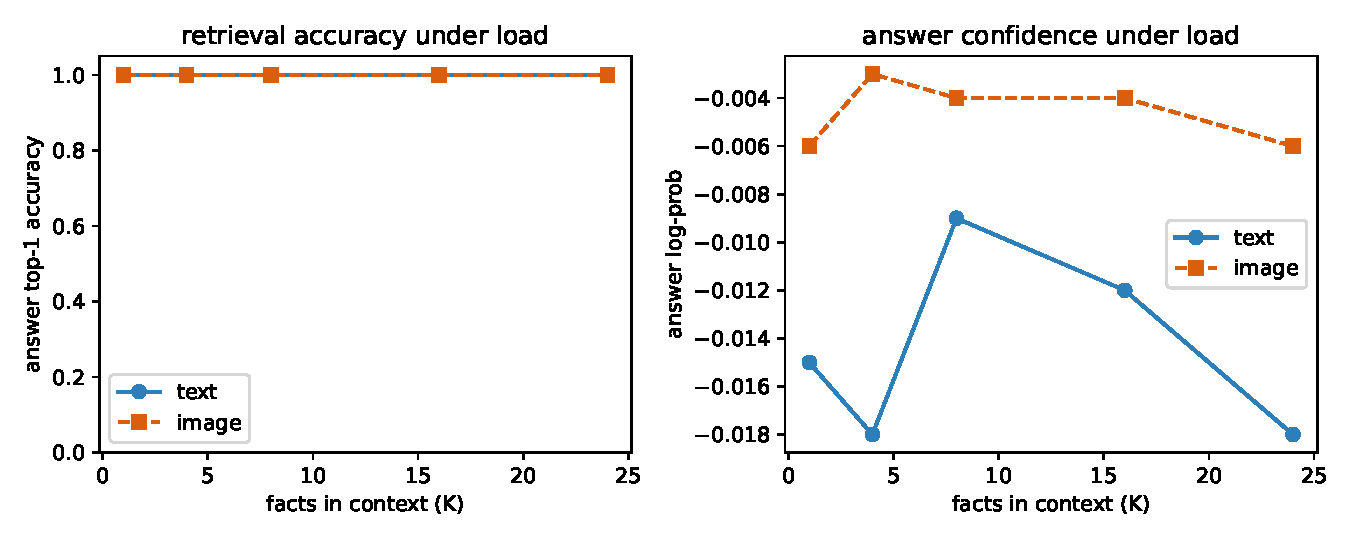
\includegraphics[width=0.88\linewidth]{figures/fig_mech_e6load.pdf}
\caption{Vision activation probe (open VLM): layer-wise logit-lens on Qwen2.5-VL-7B.}
\end{subfigure}\\[4pt]
\begin{subfigure}{\linewidth}
\centering
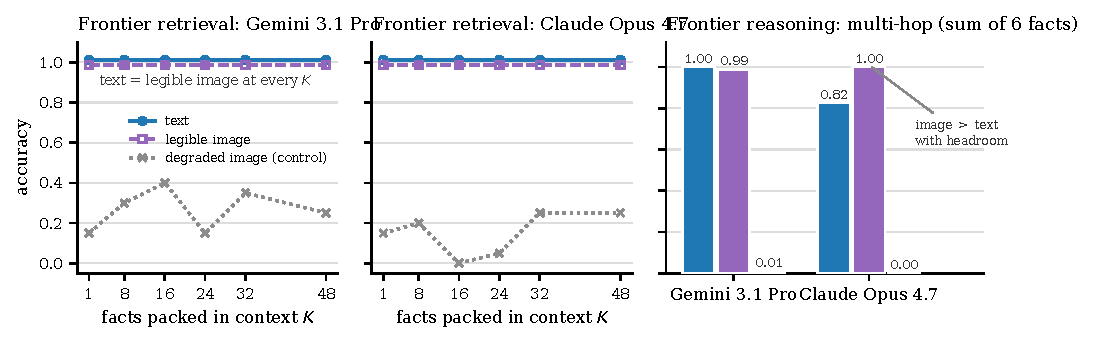
\includegraphics[width=\linewidth]{figures/fig_substrate_frontier.pdf}
\caption{Frontier probes, behavioral (the headline frontier models).}
\end{subfigure}
\caption{\textbf{Legible pixels are not a worse reasoning medium than text.} \textbf{(a)} Open VLM activation probes find equivalent text/image readout through $K\le24$ facts (within $\pm1$ layer); the intelligible-audio analogue is also null. \textbf{(b)} On the headline models, retrieval from text and legible images is identical through $K{=}48$ (pooled gap $0.000$; equivalent within $\pm0.1$); the degraded-image control drops to $0.15$--$0.27$. In multi-hop reasoning, Gemini is at ceiling and Claude performs better from images (gap $+0.175$, 95\% CI $[0.10,0.26]$).}
\label{fig:substrate}
\end{figure}

\paragraph{Not the modality.}
The claim that text is intrinsically easier to reason over than pixels or audio is contradicted at two levels (Figure~\ref{fig:substrate}). At the \emph{activation} level, a layer-wise logit lens on two open VLMs reads novel synthetic facts equally well from text and images of the same text, from one fact to 24 packed facts. An omni-model audio analogue finds the same once TTS is intelligible: the apparent gap under robotic TTS disappears with two clean neural voices. \emph{Behaviorally}, the headline models retrieve facts equally well from pixels and text through 48 packed facts; a degraded-image control confirms that the probe detects genuine deficits. In the multi-hop reasoning task, the one model with headroom performs better from images than text. These results are limited to legible propositional content and to the capable VLMs tested; Gemini is at ceiling on the reasoning probe, leaving Claude as the relevant headroom case. Within that scope, the evidence does not support a general pixel-reasoning penalty. The contrast is decisive: the same models retrieve individual facts from pixels perfectly, yet omit roughly one third of the content in end-to-end reviews. The loss is not in reading the modality.

\begin{figure}[t]
\centering
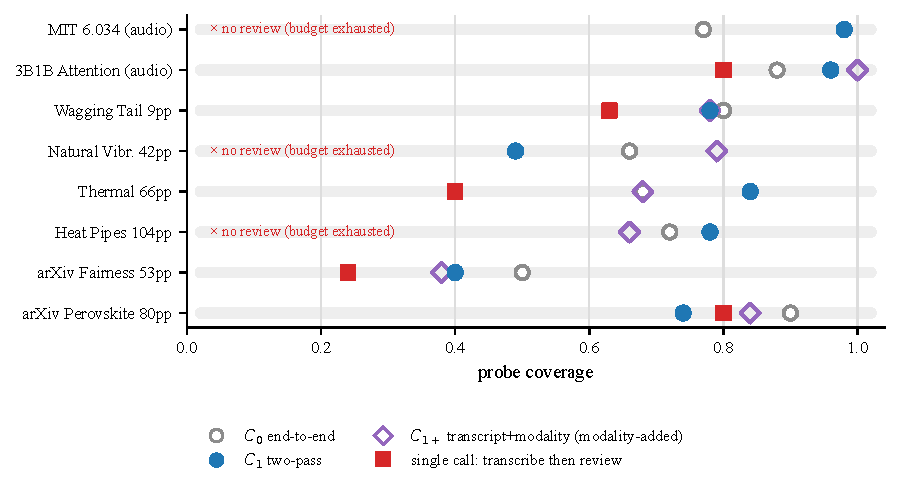
\includegraphics[width=0.82\linewidth]{figures/fig_e2_collapse.pdf}
\caption{\textbf{The benefit requires two output budgets, not removal of the modality.} On the 8-cell grid, a one-call ``transcribe then review'' prompt (red squares) usually underperforms $C_1$ and sometimes emits no review. Across 21 cells at $n{=}5$, it is lower by $\Delta_{\rm cov}{=}-0.111$ (95\% CI $[-0.170,-0.038]$; Wilcoxon $p{=}0.019$). Adding raw modality back to Pass~2 ($C_{1+}$; diamonds) leaves coverage inconclusive ($+0.069$, CI $[-0.001,+0.154]$) but adds unsupported claims on 14/21 cells.}
\label{fig:e2_collapse}
\end{figure}

\paragraph{It is generation under load.}
If merely externalizing content into the context window were sufficient, a single call that transcribed verbatim and then wrote the review should match the two-pass configuration. It does not (Figure~\ref{fig:e2_collapse}): the single call either compresses the review far below the two-pass level or spends its output budget on transcription and emits no review. The complementary modality-added control shows that raw pixels in context are not what reduce coverage. Giving Pass~2 both the transcript and the raw modality preserves the coverage benefit, but reintroduces some unsupported claims relative to text-only synthesis. The active ingredient is therefore decomposition into two passes with independent output budgets; removing the modality offers only a marginal faithfulness benefit. Appendix~\ref{appdx:substrate} reports two inconclusive controls and their confounds: DPI does not change Gemini's vision-token count, and \texttt{pdftotext} scrambles two-column reading order.

\paragraph{Verdict: perceive, externalize, synthesize.}
The evidence supports the generation-load hypothesis. The model perceives the content; the modality is not the reasoning bottleneck for legible content in our activation and behavioral tests; and recovery requires two independent output budgets, not merely text in context. A single pass asked to do everything satisfices under generation load. An externalization pass followed by a full-budget synthesis pass over complete text does not. This account predicts that the benefit will scale with the end-to-end deficit (the \emph{inverse-baseline law}, \S\ref{sec:solution}) and that decomposition will fail in two cases: when the transcript cannot fit through the synthesis output budget, and when removing the grounding source permits training-prior confabulation (\S\ref{sec:failure_modes}).

% =================================================================
\section{The solution: two-pass decomposition, and where it wins}
\label{sec:solution}

\begin{figure}[t]
\centering
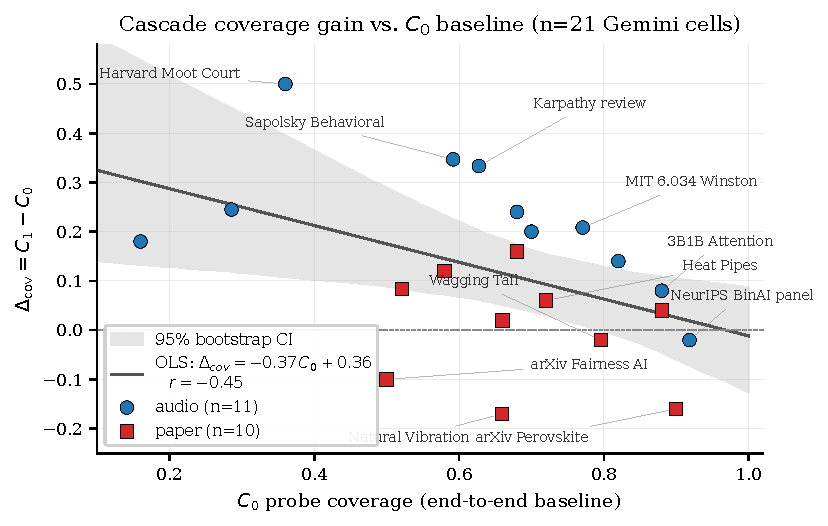
\includegraphics[width=0.62\linewidth]{figures/fig1_inverse_correlation.pdf}
\caption{\textbf{The inverse-baseline law.} Cells with weaker end-to-end coverage gain more from decomposition ($r{=}-0.45$, bootstrap 95\% CI $[-0.73,-0.10]$). Circles denote audio and squares papers; the line and band are OLS and its bootstrap CI. Counter-cells have little headroom or exhibit Modes~A/B.}
\label{fig:solution}
\end{figure}

\paragraph{The configuration.}
Figure~\ref{fig:schematic} defines the configuration motivated by \S\ref{sec:mechanism}. In $C_1$, the \emph{two-pass decomposition}, Pass~1 transcribes the source to text (perceive and externalize, using the reference-pipeline prompt) and Pass~2 writes a review from that transcript alone (synthesize). The weights are unchanged. Relative to $C_0$, the reasoning-and-writing step sees text rather than raw pixels or audio. We use four variants later: $C_{1c}$ (chunked Pass~2; $^{\rm concat}$ means no merge), $C_1^{\rm strip}$ (citation surface forms replaced with \texttt{[REF]}), $C_{1\rm iter}$ (quote-grounded iterative refinement; \S\ref{sec:failure_modes}), and $C_{1+}$ (transcript plus modality, the modality-added control).

\begin{figure}[t]
\centering
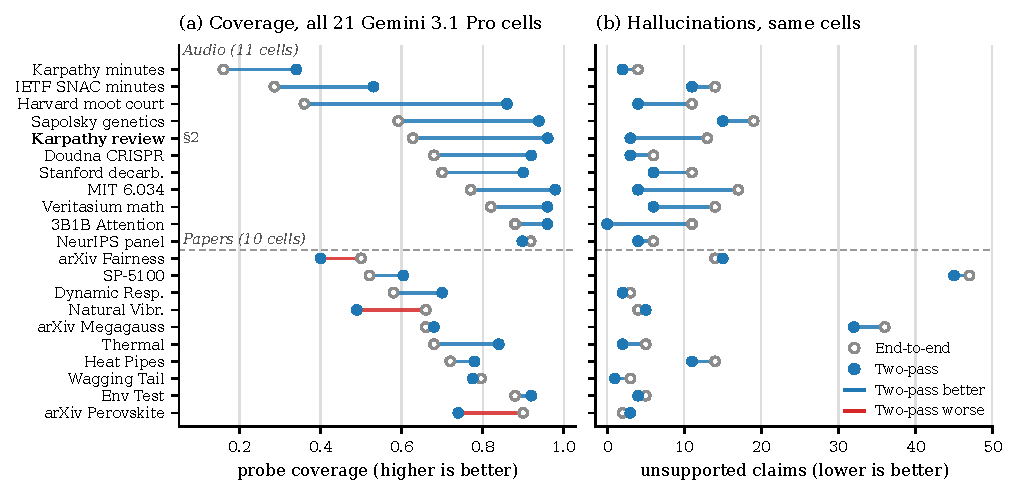
\includegraphics[width=\linewidth]{figures/fig_headline.pdf}
\caption{\textbf{Per-cell results for all 21 Gemini~3.1~Pro cells.} Cells are sorted by $C_0$ coverage within modality; the bold row is the running example. $C_1$ improves coverage on 16/21 (mean $\Delta_{\rm cov}{=}+0.118$, 95\% CI $[+0.048,+0.189]$) and reduces unsupported claims on 18/21 (mean $-3.86$, CI $[-5.62,-2.33]$). Red connectors mark regressions.}
\label{fig:headline_cells}
\end{figure}

\paragraph{Headline result at $n{=}21$.}
Figure~\ref{fig:headline_cells} shows the per-cell results behind Figure~\ref{fig:headline}. Decomposition reduces hallucinations in 18/21 cells and improves coverage in 16/21; both effects are sign-test significant. The direction remains after restricting the analysis to cells outside the noise floor and substituting medians for four cells with high judge variance (\S\ref{sec:robust}). Harvard Moot Court shows the largest coverage gain ($+50$pp), where the end-to-end baseline is weakest; 3B1B Attention shows the clearest faithfulness gain (11 unsupported claims to 0). A key caveat is that Pass~1 and the reference transcript share a model, which could favor $C_1$. An independent ASR/OCR reference preserves the direction on 4/4 cells, but this control is small; we therefore treat shared-model reference bias as the principal threat to the headline result.

\paragraph{The inverse-baseline law.}
Figure~\ref{fig:solution} shows the organizing regularity: coverage gain scales inversely with the end-to-end baseline. This is what perceive--externalize--synthesize predicts. $C_0$ coverage measures how much the monolithic pass satisfices on a cell, and the perception check shows that its omitted content is available in the transcript. Cells with more headroom can therefore recover more from a full-budget synthesis pass. This is a headroom relationship, not a promise of a universal improvement. The five counter-cells either begin near saturation (NeurIPS at $C_0{=}0.92$; Wagging Tail at roughly $0.80$) or fall into the two predicted failure regimes (\S\ref{sec:failure_modes}). Perovskite's initial $-16$pp loss shrinks to $-6$pp, near the noise floor, in $n{=}5$ re-runs (\S\ref{sec:robust}).

\begin{figure}[t]
\centering
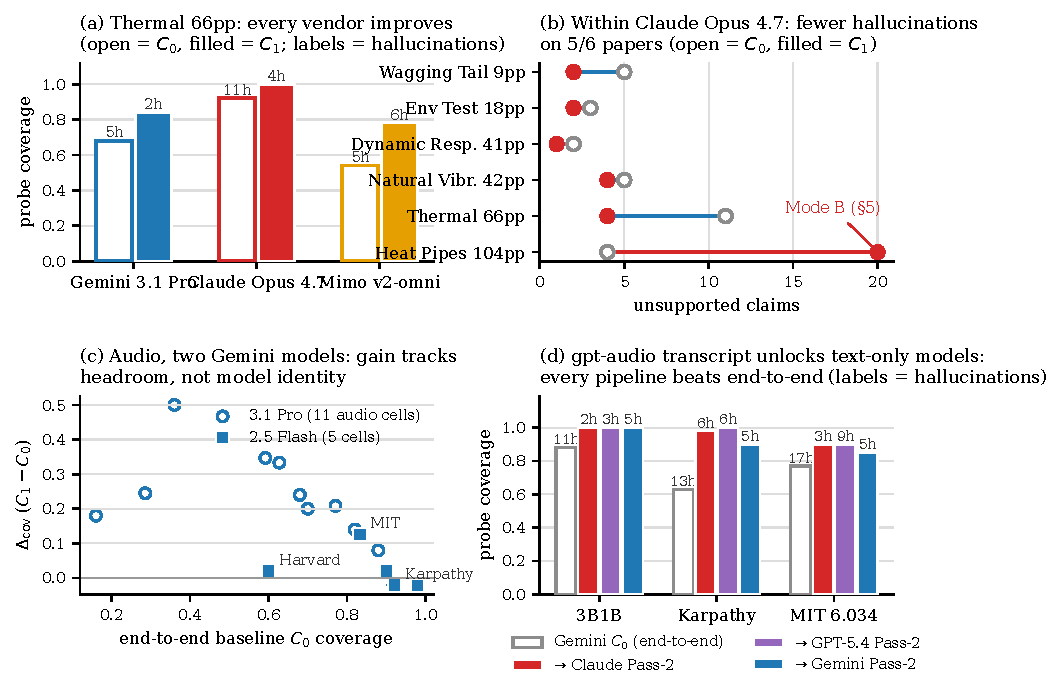
\includegraphics[width=0.98\linewidth]{figures/fig_xmodel_grid.pdf}
\caption{\textbf{Cross-model results follow the inverse-baseline law rather than replicating uniformly.} \textbf{(a)} On Thermal (66 pages), all three vendors gain coverage; Gemini and Claude converge near 1.4 unsupported claims per 1k words. \textbf{(b)} In Claude's six feasible NASA cells, hallucinations fall on 5/6; the exception is Heat Pipes (Mode~B), while short papers have little coverage headroom. \textbf{(c)} Flash's strong audio baseline leaves gains only on MIT and Harvard; Karpathy regresses. \textbf{(d)} Mixed pipelines let text-only models review audio and beat the native end-to-end baseline on both axes.}
\label{fig:xmodel}
\end{figure}

\paragraph{Cross-model and cross-vendor.}
Every cross-model result is an instance of the same law (Figure~\ref{fig:xmodel}): wins where the end-to-end baseline leaves headroom, washouts where it is already strong. We emphasize what this is \emph{not}: not a blanket vendor-independent win, and the headline aggregate remains single-vendor (Gemini). A clean cross-\emph{company} same-weights audio cascade is impossible by API constraint (no non-Google frontier model both ingests audio and accepts a text-only Pass-2; \S\ref{sec:discussion}), which is why the mixed-model pipelines of Figure~\ref{fig:xmodel}d are more deployment-relevant: in practice, different models may be used for different stages, and transcription lets text-only frontier models contribute to audio review. On long papers the vendors diverge sharply---Gemini stays small-Pareto-positive on Heat Pipes 104pp while Claude regresses on faithfulness, and on SP-5100 176pp both vendors' $C_1$ show the same bibliographic-expansion signature (Appendix~\ref{appdx:xvendor})---which is the failure-mode structure the next section dissects.

\paragraph{Cost.}
$C_1$ is $N{+}1$ calls versus one: call ratios range from ${\approx}2\times$ on short audio to ${\approx}177\times$ on the 176pp paper, with output-token volume scaling with source length (cost-vs-gain scatter in Figure~\ref{fig:cost}, \S\ref{sec:discussion}). The evidence says decomposition pays off where end-to-end has measurable headroom and buys nothing on saturated cells---so the inverse-baseline law is also the cost rule.

% =================================================================
\section{Where decomposition breaks: two failure modes and their fixes}
\label{sec:failure_modes}

The mechanism predicts two failure modes, both of which we observe. \textbf{Mode~A (compression bottleneck)} occurs when Pass~2's fixed output budget (roughly 2k words) is much shorter than the transcript, forcing synthesis to omit content. \textbf{Mode~B (training-prior leak)} occurs when removing the raw source also removes a grounding anchor, allowing Pass~2 to expand abbreviated details from prior knowledge on documents with substantial training-data overlap. Mode~B is a real but secondary cost of removing the modality; the modality-added control shows the complementary effect. Figure~\ref{fig:failure_modes}a separates the two modes by vendor on Heat Pipes (104pp).

\begin{figure}[t]
\centering
\begin{subfigure}[c]{0.38\linewidth}
\centering
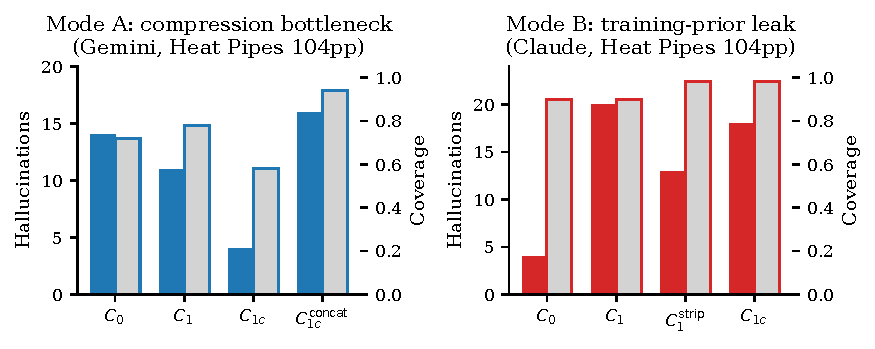
\includegraphics[width=\linewidth]{figures/fig4_failure_modes.pdf}
\caption{The two modes, on Heat Pipes (104 pages).}
\end{subfigure}\hfill
\begin{subfigure}[c]{0.60\linewidth}
\centering
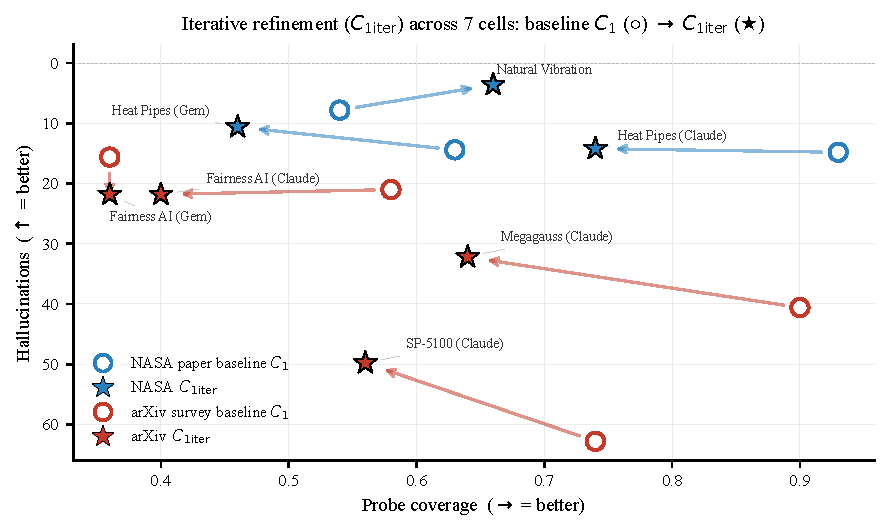
\includegraphics[width=\linewidth]{figures/fig11_iter_pareto.pdf}
\caption{$C_{1\rm iter}$ across 7 cells ($n{=}5$ means).}
\end{subfigure}
\caption{\textbf{Failure modes and iterative refinement.} \textbf{(a)} Mode~A is a Pass-2 compression bottleneck: chunking raises Heat Pipes Gemini coverage from $0.78$ to $0.94$, at five more unsupported claims. Mode~B is bibliographic confabulation: the apparent citation-strip fix is null at $n{=}5$ (CI $[-6.9,+3.3]$). \textbf{(b)} Stars show quote-grounded iterative refinement relative to plain $C_1$ (open circles): Natural Vibration is the only Pareto win; other cells trade axes or regress.}
\label{fig:failure_modes}
\end{figure}

\paragraph{Mode~A: compression bottleneck (3 papers).}
Three Gemini cells have transcript-to-budget ratios of roughly $9$--$15\times$: Heat Pipes (104pp; a small $+6$pp gain), arXiv Fairness AI (53pp; $-10$pp), and arXiv Perovskite (80pp; $-16$pp at $n{=}1$, $-6$pp under multi-seed evaluation). Our tested intervention, \textbf{chunked Pass~2}, splits the transcript into roughly 5k-word chunks, summarizes each, and concatenates the results. It raises Heat Pipes coverage from $0.78$ to $0.94$ (Figure~\ref{fig:failure_modes}a). The direction replicates at $n{=}5$ for Fairness AI and Perovskite but not Megagauss; we therefore describe it as a Mode-A intervention replicated on two of three arXiv cells (Appendix~\ref{appdx:fixes}).

\paragraph{Mode~B: training-prior leak (4 papers).}
The Heat Pipes paper cites ``Reference~2 (Cotter)''; Claude's $C_1$ expands this to ``Cotter's 1965 analysis (LA-3246-MS)''---the year and report number are training-data details absent from the transcript (more examples in Appendix~\ref{appdx:examples}). The same bibliographic-expansion signature appears on all four long, reference-dense Claude cells---Heat Pipes, SP-5100, Megagauss, and Fairness~AI, whose author--year citations (${\approx}6$ per 1k words) the numeric-form regex behind the \emph{cite/1k} feature undercounts at $0.03$---and is absent on the citation-light Thermal 66pp. Two deployment triggers emerge (thresholds and per-cell citation densities in Appendix~\ref{appdx:cell_table}): Mode~A when the transcript is $\gtrsim 5\times$ the Pass-2 output budget and the coverage gain is small; Mode~B when the source carries $\gtrsim 2$ citation surface forms per 1k words in \emph{any} style \emph{and} its cited literature is widely represented pre-cutoff (true of Fairness~AI's fairness canon even though the paper itself is post-cutoff). The modes compound (Mimo Heat Pipes shows both) or occur alone (Heat Pipes: Gemini dominantly A, Claude dominantly B).

\begin{figure}[!t]
\centering
\begin{subfigure}{0.495\linewidth}
\centering
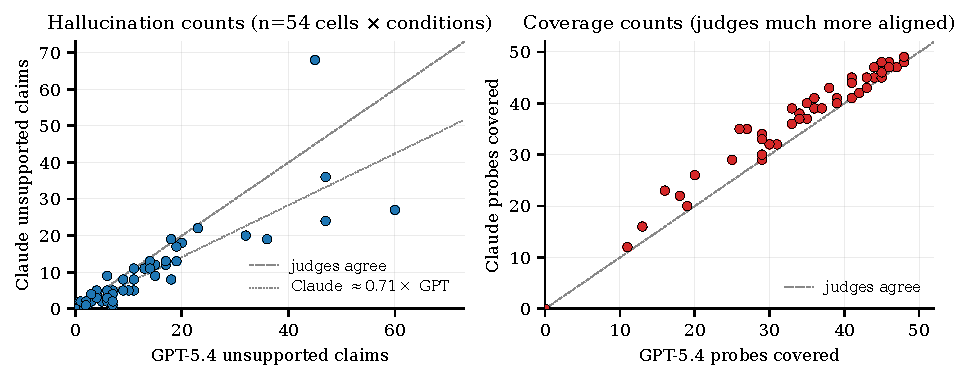
\includegraphics[width=\linewidth]{figures/fig10_inter_judge_scatter.pdf}
\caption{Inter-judge replication, all 21 cells ($+$1 cross-vendor).}
\end{subfigure}\hfill
\begin{subfigure}{0.475\linewidth}
\centering
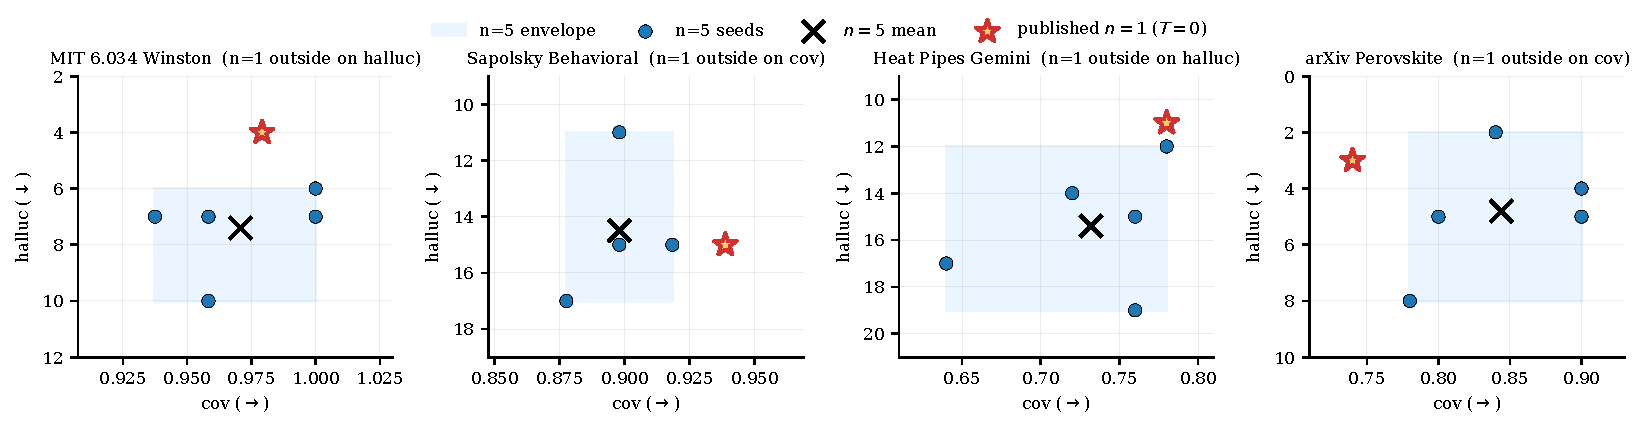
\includegraphics[width=\linewidth]{figures/fig12_headline_multiseed.pdf}
\caption{$n{=}5$ Pass-2 multi-seed envelopes.}
\end{subfigure}\\[4pt]
\begin{subfigure}{0.50\linewidth}
\centering
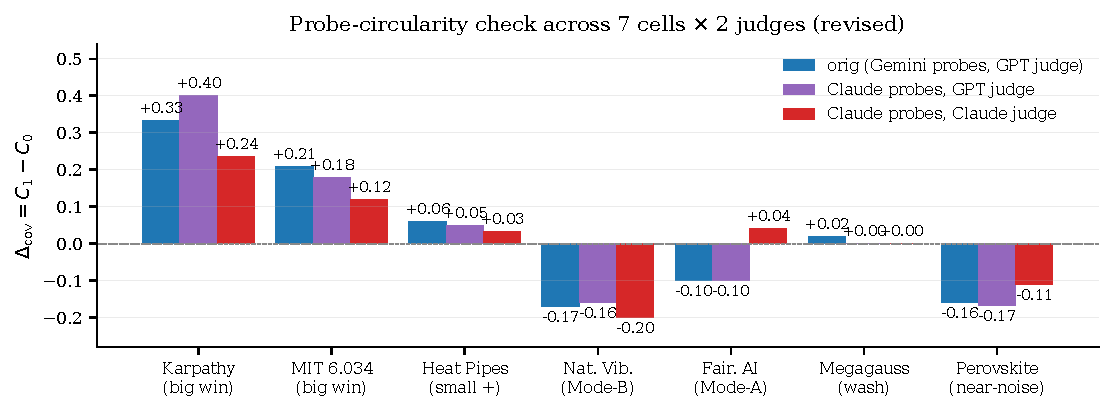
\includegraphics[width=\linewidth]{figures/fig8_probe_circularity.pdf}
\caption{Probe re-extraction (7 cells).}
\end{subfigure}\hfill
\begin{subfigure}{0.47\linewidth}
\centering
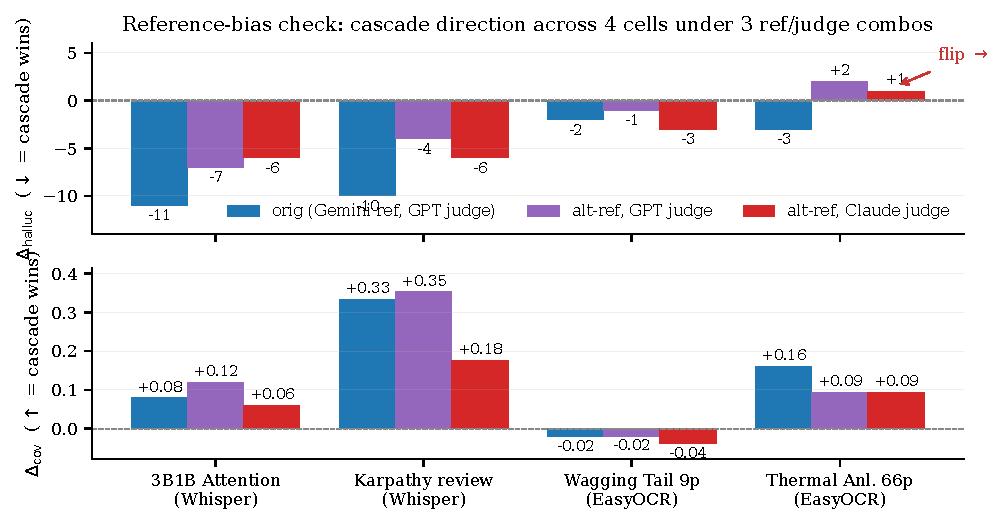
\includegraphics[width=\linewidth]{figures/fig9_reference_bias.pdf}
\caption{Independent reference (4 cells).}
\end{subfigure}
\caption{\textbf{Four robustness checks.} \textbf{(a)} A Claude Opus 4.7 re-judge agrees with GPT-5.4 on 19/21 coverage and 14/21 hallucination directions (median per-probe agreement $0.94$). \textbf{(b)} Across five Pass-2 seeds, three headline wins preserve direction; Perovskite's loss shrinks to $-6$pp. \textbf{(c)} After Claude re-extracts probes, coverage direction is preserved on 6/7 cells under GPT-5.4 and 5/7 under Claude. \textbf{(d)} Independent ASR/OCR preserves coverage direction on all four cells; EasyOCR's lone hallucination flip reflects missing figure captions.}
\label{fig:robustness}
\end{figure}

\paragraph{Citation stripping does not replicate.}
Beyond chunked Pass~2, we tested \emph{citation stripping} ($C_1^{\rm strip}$) as a Mode-B intervention. \textbf{It does not survive replication.} The original Heat Pipes estimate ($20\to13$) falls within the combined Pass-2 and judge-noise envelope at $n{=}5$, and the intervention produces no replicated win across four cells (Appendix~\ref{appdx:fixes}). We therefore do not treat citation stripping as an effective Mode-B intervention. We next evaluate a quote-grounded refinement that addresses Mode~B structurally.

\paragraph{$C_{1\rm iter}$: a quote-grounded refinement.}
Mode~B calls for re-grounding synthesis in the transcript. $C_{1\rm iter}$ (a) extracts 50--150 atomic claims, each with a verbatim quote of at most 25 words; (b) removes claims whose quotes do not fuzzy-match the transcript; and (c) rewrites the review using the remaining claims. The filter is a tripwire rather than a culler: $99.8\%$ of claims pass ($3731/3738$). Requiring a quote appears to discourage the bibliographic expansions characteristic of Mode~B. This applies RAG-style attribution discipline within a same-weights self-cascade. At $n{=}5$ across seven cells (Figure~\ref{fig:failure_modes}b), its result depends on the dominant failure mode: it suppresses Mode~B where Mode~B is binding, but imposes a rewrite-compression cost. It is therefore Pareto-positive only when the rewrite does not over-compress.


% =================================================================
\section{Robustness}
\label{sec:robust}


Figure~\ref{fig:robustness} summarizes four checks against the main protocol threats: judge idiosyncrasy (a), Pass-2 and judge stochasticity (b), probe circularity---GPT-5.4 both extracts and scores the probes (c)---and shared-model reference bias (d). The last is the principal residual threat. Although the independent-reference control preserves direction in all four cells, it is small and concentrated on strong-win cases.

\begin{figure}[!t]
\centering
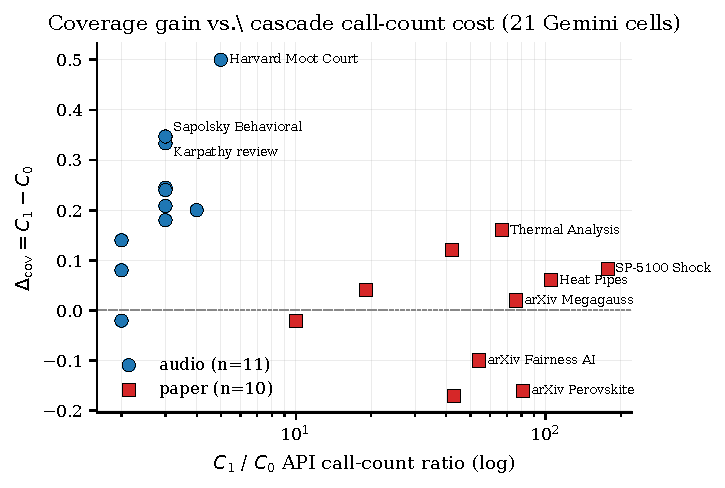
\includegraphics[width=0.6\linewidth]{figures/fig5_cost_pareto.pdf}
\caption{\textbf{Coverage gain versus API call-count cost.} Each point is a Gemini cell. Paper $C_1/C_0$ ratios are $N{+}1$ (one OCR call per page plus Pass~2), versus roughly $2$--$3\times$ for chunked audio ASR. Gains are generally largest for cheap audio and smaller for costly papers, but baseline headroom explains exceptions such as SP-5100.}
\label{fig:cost}
\end{figure}

Separating stochasticity sources (Figure~\ref{fig:stoch}; Appendix~\ref{appdx:stoch}) yields three operational conclusions. Pass~2 generation varies: Claude no longer exposes a temperature parameter, and Gemini at $T{=}0$ is mostly, but not perfectly, deterministic. GPT-5.4 is effectively deterministic on low-count cells but varies by $\pm10$--$25$ on long unsupported-claim lists that approach its completion budget. Coverage is substantially more stable than hallucination counts under all three sources of variation. We therefore use medians for the four high-count cells in the headline aggregates and flag hallucination counts above roughly 30 as judge-uncertain. Crucially, the Mode-B \emph{observation} survives these checks, whereas citation stripping does not demonstrate a reliable intervention effect. A four-feature leave-one-out logistic predictor of $\mathrm{sign}(\Delta_{\rm cov})$ reaches AUC $0.65$, an informative $n{=}21$ baseline but not a deployment-ready model (Appendix~\ref{appdx:cell_table}).


% =================================================================
\section{Related work}
\label{sec:related}

\paragraph{Speech and documents.} Prior cascade-vs-end-to-end results are often read as modality claims; our mechanism study suggests they are at least partly about decomposition and modality-specific recoverability. Cuervo et al.~\cite{cuervo2025closing} document a text/speech understanding gap, and the Cascade Equivalence Hypothesis~\cite{ceh2026} shows speech-LLMs \emph{internally} behave like ASR$\to$LLM cascades, while X-Talk~\cite{xtalk2025} finds explicitly cascaded speech-to-speech pipelines competitive. On documents, DocVLM~\cite{docvlm2024} reports OCR-augmented VLMs beating pure-vision VLMs on DocVQA at fixed budget, while the OCR-Reasoning Benchmark~\cite{ocrreasoning2026} shows pure-OCR cascades cap below 50\% where spatial layout carries meaning, ColPali~\cite{colpali2025} shows vision-only retrieval beating OCR, and GUI agents do better from raw pixels than from structured-text intermediates~\cite{uground2024,uitars2025}. A parallel vision-side literature isolates the modality by rendering identical content as text versus as an \emph{image} of that text: VISTA-Bench~\cite{vistabench2026} finds a pronounced gap across 20+ open VLMs but a near-zero gap on the strongest models---including Qwen2.5-VL ($-2.0$ points), the model in our vision activation probe---consistent with our modality null (\S\ref{sec:mechanism}), while CrossMath~\cite{crossmath2026} bounds it: on 2D symbolic-arithmetic grids, reasoning from an \emph{image} collapses relative to a markdown-table rendering of the same grid ($12.4$ vs.\ $92.8$ on Qwen3.5-Plus) with OCR intact. Its authors attribute this to a modality deficit; we read the same numbers---and the fact that serializing the identical layout to text restores reasoning---as a penalty specific to recovering 2D structure from pixels rather than to legible content per se. The common thread matches our mechanism: decomposition helps when the task is generation-under-load and the content survives transcription, and hurts when the answer lives in layout or signal that transcription discards.

\begin{table}[!t]
\small
\centering
\caption{\textbf{Practitioner checklist} drawn from this paper's cells: which configuration to deploy per source/model regime.}
\label{tab:checklist}
\begin{tabular}{p{0.34\linewidth}p{0.30\linewidth}p{0.27\linewidth}}
\toprule
Source / model class & Diagnosis & Recommended action \\
\midrule
Audio talk or moderate paper (40--70pp) on a capable model & Cascade strongly Pareto-positive. & Default $C_1$. \\
Moderate paper with Mode-B Gemini signature (Natural~Vibration~42pp) & Mode~B dominant, and the cell flips to Pareto-positive under $C_{1\rm iter}$. & $C_{1\rm iter}$. \\
Long paper, Mode~A dominant (Heat~Pipes~104pp Gemini) & Compression bottleneck. & $C_{1c}^{\rm concat}$ (chunked, no merge). \\
Long paper, Mode~B dominant (Heat~Pipes Claude) & Citation-prior leak, but the $C_{1\rm iter}$ faithfulness gain washes out at $n{=}5$. & $C_0$ if it fits. $C_{1\rm iter}$ buys only a coverage loss. \\
Long survey (arXiv Fairness~AI, Megagauss; NASA SP-5100) & Mode~A + Mode~B compound. At $n{=}5$, $C_{1\rm iter}$ is net-negative on Fairness~AI but a faithfulness/coverage trade on SP-5100/Megagauss. Chunked Pass-2 partially replicates. & Prefer $C_0$ when it fits. If cascade required, use $C_{1c}^{\rm concat}$ with multi-seed averaging. \\
\bottomrule
\end{tabular}
\end{table}

\paragraph{Step-Audio-R1: a boundary, not a contradiction.} Step-Audio-R1~\cite{stepaudior1} observes audio LLMs spontaneously reasoning over a \emph{textual surrogate} of the audio (attributing musical sadness to ``lyrics mention sadness'' rather than a minor key) and treats this as the failure its modality-grounded distillation must correct. Their tasks---music, environmental sound, paralinguistics---have \emph{acoustic} answers that transcription discards; ours is the complementary regime, where the payload is what was \emph{said}. Our activation tests find no modality gap for propositional content in either modality (the activation probes), so we read their effect as task-payload-specific rather than as ``audio is a worse modality.'' Our Mode~B is the within-regime echo of their concern.

\paragraph{Cascade theory and faithfulness.} Bengio's Consciousness Prior~\cite{bengio2017consciousness} argues for sparse discrete bottlenecks between perception and reasoning; our externalized text bottleneck is a deployment-time analogue, and Discrete JEPA~\cite{discretejepa2025} makes a related architectural argument within vision. Mode~B is a self-cascade analogue of the unfaithfulness problem motivating RAG~\cite{rag2020}, RARR~\cite{rarr2023}, and Attribution to Identified Sources~\cite{ais2022}; $C_{1\rm iter}$ adopts RARR's in-context-attribution discipline but operates entirely within a same-weights self-cascade without external retrieval.

% =================================================================
\section{Discussion and limitations}
\label{sec:discussion}

\paragraph{What generalizes.} The portable result is not that decomposition always wins, but the inverse-baseline law: it recovers more content when end-to-end review leaves more content unrecovered. It is therefore most useful where a model performs poorly on the raw modality and offers little benefit where the baseline is already strong. This makes the cross-vendor results coherent rather than contradictory: Claude's near-ceiling NASA papers, Gemini~2.5~Flash's strong end-to-end audio, and Gemini~Pro's weaker end-to-end audio follow the same relationship (Figure~\ref{fig:xmodel}). The most deployable implication is that transcription lets text-only frontier models contribute to audio review (Figure~\ref{fig:xmodel}d). Table~\ref{tab:checklist} summarizes the recommended configuration for each regime.

\begin{figure}[!t]
\centering
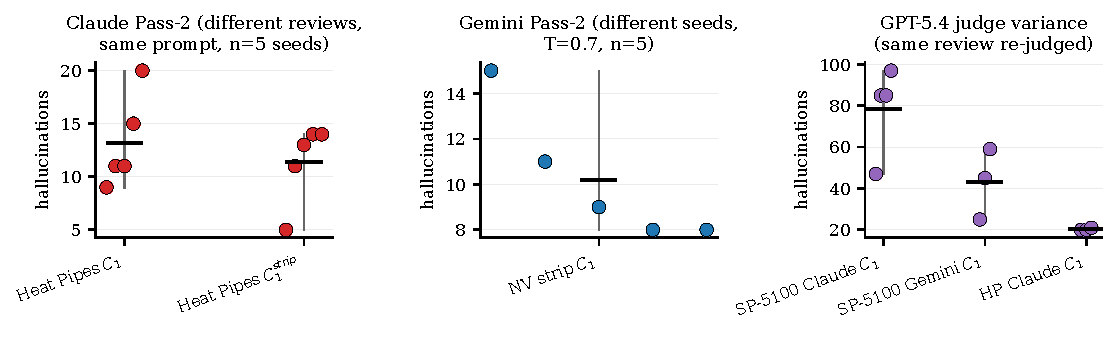
\includegraphics[width=\linewidth]{figures/fig7_stochasticity.pdf}
\caption{\textbf{Three sources of stochasticity.} Left and middle: Pass-2 generation variance for Claude and Gemini. Right: GPT-5.4 re-judging the same review. Hallucination counts vary much more than coverage, particularly for high-count SP-5100.}
\label{fig:stoch}
\end{figure}

\paragraph{Limitations.}
\emph{Scope:} the headline aggregate is single-vendor; the within-Claude comparison replicates the faithfulness direction on 5/6 papers but is not independently significant at $n{=}6$, and Claude $C_0$ is unrealizable beyond 104pp. A cross-company same-weights \emph{audio} cascade is impossible due to API constraints (Claude takes no audio; OpenAI's audio model refuses text-only Pass-2), so the mixed pipeline is the natural production form. The Mimo audio cells ran at reduced bitrate (OpenRouter cap), conflating quality with model weakness; the full-quality 2.5~Flash arm removes that confound and is headroom-gated as predicted.
\emph{Measurement:} probe and reference bias are only partially controlled (7 and 4 cells); the shared-model reference remains the principal threat to the headline statistic; single-judge intra-rater variance affects high-count cells ($\pm10$--$25$; Figure~\ref{fig:stoch}). Several sources predate the model cutoff, but memorization biases \emph{against} the cascade (it aids $C_0$), making the headline conservative; the post-cutoff sources span wins and counter-cells, consistent with the law.
\emph{Mechanism breadth:} all measurements concern long-form review; we make no claim about short-form QA, code, or agentic tasks. The frontier probes are behavioral rather than activation-level because frontier activations are inaccessible. Gemini is at ceiling on the reasoning probe, leaving Claude as the only headroom case. We have not tested real scanned or degraded pages (the degraded control is synthetic), and the DPI and reading-order controls are single-seed and confounded.

\paragraph{Validation plan.}
The load-bearing effects are already multi-seed on all 21 cells, so remaining replication is about breadth, not statistical power: extend the vision activation probe to other open families and, where activations become accessible, lift the frontier probes to the activation level; push the audio activation probe into the multi-fact load regime; re-test on real scanned and degraded pages, where a modality or dilution effect is most likely to appear; extend to other generation-under-load tasks plus a short-form control where the account predicts \emph{no} decomposition benefit; and causally vary the synthesis output budget to confirm Mode~A is budget-bound.

% =================================================================
\section{Conclusion}
\label{sec:conclusion}

For long-form review, the intuitive end-to-end deployment of a multimodal model quietly satisfices: it omits roughly one third of content that the same model can transcribe and adds unsupported detail. Our evidence points to generation under load rather than a general perception or modality deficit. Open models read text and images of the same text equally well at the activation level, and frontier models do so behaviorally; the difficulty is asking one pass to perceive, reason, and write a long faithful review simultaneously. A same-weights, two-pass decomposition with independent output budgets improves faithfulness and coverage across 21 cells and follows an inverse-baseline law: it helps most where the monolithic pass leaves the most headroom. Its two predicted failure modes---synthesis-budget overflow and source-removal confabulation---also appear. Chunked Pass~2 and quote-grounded refinement provide partial, condition-dependent remedies. The practical rule is \textbf{perceive, externalize, then synthesize}: a deployment pattern with predictable failure modes, not a universal architecture.

% =================================================================
\section*{Acknowledgements}

This paper was produced using Pine Copilot's voice-directed \emph{whisper coding} workflow~\cite{pineai2026whispercoding}, in which the authors specify, discuss, and review the work by voice while a coding agent---Claude Code with Claude Opus 4.8---carries out the planning, coding, experiments, and paper writing.
We thank BSQL Networking for hosting the NVIDIA RTX PRO 6000 GPU.

% =================================================================
\bibliographystyle{plainnat}
\begin{thebibliography}{99}

\bibitem{pineai2026whispercoding}
{Pine AI}.
\newblock {Pine AI}: the most natural human-computer interface is your voice.
\newblock Blog post, 2026.
\newblock \url{https://www.19pine.ai/blog/pine-ai-the-most-natural-human-computer-interface-is-your-voice}. Accessed 2026-06-28.

\bibitem{cuervo2025closing}
S.~Cuervo, S.~Seto, M.~de~Seyssel, R.~H.~Bai, Z.~Gu, T.~Likhomanenko, N.~Jaitly, and Z.~Aldeneh.
\newblock Closing the gap between text and speech understanding in LLMs.
\newblock {\em arXiv preprint arXiv:2510.13632}, 2025.

\bibitem{ceh2026}
J.~Billa.
\newblock The cascade equivalence hypothesis: when do speech LLMs behave like ASR$\to$LLM pipelines?
\newblock {\em arXiv preprint arXiv:2602.17598}, 2026.

\bibitem{xtalk2025}
Z.~Liu, Y.~Duan, M.~Wang, P.~Feng, H.~Zhang, X.~Xing, Y.~Shan, H.~Zhu, Y.~Dai, C.~Lu, X.~Qiu, L.~Xie, L.~Wang, N.~Yan, Z.~Zheng, Z.~Ma, K.~Yu, and X.~Chen.
\newblock X-{T}alk: on the underestimated potential of modular speech-to-speech dialogue systems.
\newblock {\em arXiv preprint arXiv:2512.18706}, 2025.

\bibitem{stepaudior1}
F.~Tian, X.~T.~Zhang, Y.~Zhang, H.~Zhang, Y.~Li, D.~Liu, Y.~Deng, D.~Wu, J.~Chen, L.~Zhao, C.~Yao, H.~Liu, E.~S.~Chng, X.~Yang, X.~Zhang, D.~Jiang, and G.~Yu.
\newblock Step-{A}udio-{R}1 technical report.
\newblock {\em arXiv preprint arXiv:2511.15848}, 2025.

\bibitem{docvlm2024}
M.~Shpigel Nacson, A.~Aberdam, R.~Ganz, E.~Ben Avraham, A.~Golts, Y.~Kittenplon, S.~Mazor, and R.~Litman.
\newblock {DocVLM}: make your {VLM} an efficient reader.
\newblock {\em arXiv preprint arXiv:2412.08746}, 2024.

\bibitem{vistabench2026}
Q.~Liu, J.~Feng, Y.~Wang, X.~Han, Y.~Cheng, Y.~Zhu, H.~Diao, Y.~Zhuge, and H.~Lu.
\newblock {VISTA-Bench}: do vision-language models really understand visualized text as well as pure text?
\newblock {\em arXiv preprint arXiv:2602.04802}, 2026.

\bibitem{crossmath2026}
Y.~Xu, Y.~Wang, Z.~Wu, K.~Song, J.~Lin, and Z.~Shen.
\newblock Do vision-language models truly perform vision reasoning? {A} rigorous study of the modality gap.
\newblock {\em arXiv preprint arXiv:2604.16256}, 2026.

\bibitem{ocrreasoning2026}
M.~Huang, Y.~Shi, D.~Peng, S.~Lai, Z.~Xie, and L.~Jin.
\newblock {OCR}-{R}easoning benchmark: unveiling the true capabilities of {MLLMs} in complex text-rich image reasoning.
\newblock {\em arXiv preprint arXiv:2505.17163}, 2025.

\bibitem{colpali2025}
M.~Faysse, H.~Sibille, T.~Wu, B.~Omrani, G.~Viaud, C.~Hudelot, and P.~Colombo.
\newblock {ColPali}: efficient document retrieval with vision language models.
\newblock In {\em International Conference on Learning Representations ({ICLR})}, 2025.
\newblock arXiv:2407.01449.

\bibitem{uground2024}
B.~Gou, R.~Wang, B.~Zheng, Y.~Xie, C.~Chang, Y.~Shu, H.~Sun, and Y.~Su.
\newblock Navigating the digital world as humans do: universal visual grounding for {GUI} agents.
\newblock {\em arXiv preprint arXiv:2410.05243}, 2024.

\bibitem{uitars2025}
H.~Wang, H.~Zou, H.~Song, J.~Feng, J.~Fang, J.~Lu, L.~Liu, Q.~Luo, S.~Liang, S.~Huang, W.~Zhong, Y.~Ye, Y.~Qin, Y.~Xiong, Y.~Song, Z.~Wu, et~al.
\newblock {UI}-{TARS}-2 technical report: advancing {GUI} agents with multi-turn reinforcement learning.
\newblock {\em arXiv preprint arXiv:2509.02544}, 2025.

\bibitem{bengio2017consciousness}
Y.~Bengio.
\newblock The consciousness prior.
\newblock {\em arXiv preprint arXiv:1709.08568}, 2017.

\bibitem{discretejepa2025}
J.~Baek, H.~Lee, C.~Hoang, M.~Ren, and S.~Ahn.
\newblock Discrete {JEPA}: learning discrete token representations without reconstruction.
\newblock In {\em ICML 2025 Tokenization Workshop ({TokShop})}, 2025.
\newblock arXiv:2506.14373.

\bibitem{rag2020}
P.~Lewis, E.~Perez, A.~Piktus, F.~Petroni, V.~Karpukhin, N.~Goyal, H.~K\"uttler, M.~Lewis, W.-t.~Yih, T.~Rockt\"aschel, S.~Riedel, and D.~Kiela.
\newblock Retrieval-augmented generation for knowledge-intensive {NLP} tasks.
\newblock In {\em Advances in Neural Information Processing Systems ({NeurIPS})}, 2020.
\newblock arXiv:2005.11401.

\bibitem{rarr2023}
L.~Gao, Z.~Dai, P.~Pasupat, A.~Chen, A.~T.~Chaganty, Y.~Fan, V.~Y.~Zhao, N.~Lao, H.~Lee, D.-C.~Juan, and K.~Guu.
\newblock {RARR}: researching and revising what language models say, using language models.
\newblock In {\em Proceedings of the 61st Annual Meeting of the Association for Computational Linguistics ({ACL})}, 2023.
\newblock arXiv:2210.08726.

\bibitem{ais2022}
H.~Rashkin, V.~Nikolaev, M.~Lamm, L.~Aroyo, M.~Collins, D.~Das, S.~Petrov, G.~S.~Tomar, I.~Turc, and D.~Reitter.
\newblock Measuring attribution in natural language generation models.
\newblock {\em arXiv preprint arXiv:2112.12870}, 2021.

\end{thebibliography}

% =================================================================
\appendix
\section{Mechanistic experiments and controls, in detail}
\label{appdx:substrate}

This appendix expands the mechanism sections (the perception check of \S\ref{sec:observation}, and the decomposition controls, modality probes, and confounded controls of \S\ref{sec:mechanism}) with the per-experiment tables.

\paragraph{Perception check: perception is not the bottleneck.}
The per-cell breakdown is Figure~\ref{fig:mech_e3} (main text). The transcript covers a mean $99.9\%$ of probes, versus $65\%$ for the $C_0$ review and $77\%$ for $C_1$ synthesis; $361/362$ probes dropped by $C_0$ are present in the model's own transcript.

\paragraph{Vision activation probe: no cross-modal gap at the activation level.}
We tested the modality hypothesis directly on an open VLM (Qwen2.5-VL-7B), controlling for prior knowledge with novel synthetic facts about nonsense entities (e.g.\ ``the Zorblatt device weighs 7 kilograms''). Each fact is presented either as digital text or as an \emph{image} of that same text, with a matched single-token question, and a layer-wise logit-lens reads off the log-probability and rank of the answer token at every layer. The two modalities are indistinguishable for an isolated fact and under load: packing $K\in\{1,4,8,16,24\}$ facts into one stimulus, image and text stay at $1.00$ accuracy with a readout-depth gap $<1$ layer (TOST-equivalent within $\pm 1$ layer) at every $K$ (Figure~\ref{fig:substrate}a). The same null replicates on Qwen2.5-VL-3B; the per-$K$ ladder for both models is in Appendix~\ref{appdx:vision_ladder}. (The 32B variant verbalizes answers in a form our single-token matcher cannot score, so it is excluded.)

\paragraph{Audio activation probe: no audio modality gap either, once the speech is intelligible.}
We replicate the vision activation probe's logit-lens on an omni model (Qwen2.5-Omni Thinker), presenting each novel fact as text vs as \emph{synthesized speech}, across three TTS engines of increasing quality (Table~\ref{tab:e7}). The result is a methodological caution turned finding: with low-quality TTS (espeak, only $71\%$ of clips intelligible to the model's own ASR) audio \emph{appears} to have a modality gap, but this tracks \emph{intelligibility}, not modality---with two independent clean neural voices ($88\%$ and $96\%$ intelligible) the gap vanishes and is TOST-equivalent within $\pm 1$ layer. Garbled TTS manufactures a spurious gap, so audio-modality claims must control for TTS intelligibility.

\begin{table}[h]
\small\centering
\caption{Audio activation probe readout (Qwen2.5-Omni Thinker, 24 novel facts): the apparent audio modality gap is a TTS-intelligibility artifact. ``Intellig.'': fraction of clips the model's own ASR transcribes correctly. Depth-gap = audio$-$text readout depth (layers). TOST SESOI $\pm 1$ layer.}
\label{tab:e7}
\setlength{\tabcolsep}{4pt}
\begin{tabular}{lccccc}
\toprule
TTS & intellig. & text acc & audio acc & depth-gap 90\% CI & TOST-equivalent \\
\midrule
espeak (robotic)        & 0.71 & 0.96 & 0.83 & $[0.64, 1.78]$ & no (spurious gap) \\
\texttt{mms-tts-eng} (clean)   & 0.88 & 0.96 & 1.00 & $[0.18, 0.57]$ & \textbf{yes} \\
\texttt{fish-speech-1.5} (natural) & 0.96 & 0.96 & 1.00 & $[0.21, 0.54]$ & \textbf{yes} \\
\bottomrule
\end{tabular}
\end{table}

\paragraph{Frontier retrieval probe (behavioral).}
The activation probes establish the modality null only on small open models (the lens needs activations). The frontier retrieval probe closes the gap behaviorally on the exact headline models: pack $K\in\{1,8,16,24,32,48\}$ novel nonsense-entity facts (distinct two-digit values, so prior knowledge gives no shortcut) as text or as an image of that text, and ask a single-number question about one target entity ($T{=}20$ seeded trials/cell). Table~\ref{tab:e8} gives the counts behind Figure~\ref{fig:substrate}b: on both models, legible-image accuracy equals text accuracy exactly at every $K$ up to 48, while the degraded positive control (small font, downscaled and blurred to low-DPI-scan quality) collapses and is decisively non-equivalent---the probe is sensitive.

\begin{table}[h]
\small\centering
\caption{Frontier retrieval probe: behavioral cross-modal test ($T{=}20$ seeded trials per $K$, single-number retrieval). ``legible img'': image of the same text at $34$px. ``degraded img'': small-font, downscaled+blurred low-DPI-scan control. Gap = image$-$text accuracy; TOST SESOI $\pm 0.1$.}
\label{tab:e8}
\setlength{\tabcolsep}{4pt}
\begin{tabular}{llcccc}
\toprule
Model & cond & acc @ $K{=}1$ & acc @ $K{=}48$ & pooled gap (95\% CI) & TOST-equiv \\
\midrule
\multirow{3}{*}{Gemini 3.1 Pro} & text          & 1.00 & 1.00 & --- & --- \\
                                & legible img   & 1.00 & 1.00 & $+0.000$ $[0.00,0.00]$ & \textbf{yes} \\
                                & degraded img  & 0.15 & 0.25 & $-0.733$ $[-0.81,-0.65]$ & no (control) \\
\midrule
\multirow{3}{*}{Claude Opus 4.7} & text         & 1.00 & 1.00 & --- & --- \\
                                 & legible img  & 1.00 & 1.00 & $+0.000$ $[0.00,0.00]$ & \textbf{yes} \\
                                 & degraded img & 0.15 & 0.25 & $-0.850$ $[-0.91,-0.78]$ & no (control) \\
\bottomrule
\end{tabular}
\end{table}

\paragraph{Frontier reasoning probe (multi-hop).}
The frontier reasoning probe forces composition: the model must pull $M{=}6$ specified facts out of a $K$-fact packed set and \emph{sum} them---the total is never a visible number---as text vs.\ legible image vs.\ the frontier retrieval probe's degraded control ($T{=}20$/cell over $K\in\{8,16,24,32\}$, Table~\ref{tab:e9}). On Gemini, text and legible image are both at ceiling and TOST-equivalent (gap $-0.013$). On Claude without extended thinking---the one sub-ceiling regime we could produce (text accuracy $0.825$; we could not drive clean-text Gemini below ceiling at any difficulty tried)---the legible image is reliably \emph{better} (image $1.00$, gap $+0.175$, 95\% CI $[0.10,0.26]$); the $14/80$ text errors are near-miss arithmetic slips that the image condition gets right. We read the Claude effect as a within-prompt echo of this paper's thesis---reading from an image nudges the model to externalize the numbers before summing---but report only the direction.

\begin{table}[h]
\small\centering
\caption{Frontier reasoning probe: retrieve $M{=}6$ packed facts and sum them (answer never directly visible), $T{=}20$/cell over $K\in\{8,16,24,32\}$. Gap = image$-$text accuracy; TOST SESOI $\pm 0.1$.}
\label{tab:e9}
\begin{tabular}{lcccc}
\toprule
Model & text acc & legible-img acc (gap) & TOST-equiv & degraded-img acc \\
\midrule
Gemini 3.1 Pro  & 1.00  & 0.99 ($-0.013$) & \textbf{yes} & 0.01 \\
Claude Opus 4.7 & 0.825 & \textbf{1.00 ($+0.175$)} & no (image \emph{better}) & 0.00 \\
\bottomrule
\end{tabular}
\end{table}

\paragraph{DPI and reading-order controls: they did not separate the hypotheses.}
The DPI control sought to vary vision-token count via DPI on a fixed document to probe the attention-dilution hypothesis. But Gemini normalizes images internally, so $96$ and $200$ DPI yield near-identical prompt token counts ($112{,}007$ vs $111{,}855$ on Heat~Pipes); the manipulation does not move the independent variable, and the attention-dilution hypothesis is untestable this way on Gemini. The reading-order control fed native digital text (\texttt{pdftotext}) to a single text-only call as a clean modality-hypothesis test, but on two-column arXiv PDFs \texttt{pdftotext} scrambles reading order, so native-text coverage is confounded downward (Fairness~AI $0.34$, below even $C_0$). Neither supports the modality hypothesis, so we report both with their confounds rather than omit them.

\begin{table}[h]
\small\centering
\caption{Mechanistic conditions on the 8-cell subset (hallucinations\,h / probe-coverage); the data behind Figure~\ref{fig:e2_collapse}. $C_0$: end-to-end (modality). $C_1$: two-pass decomposition (text). $C_{1+}$: synthesis pass given both transcript and modality (modality-added control). single-call: transcribe-then-review in one response (single-call test, ``--'' = no review emitted, budget exhausted). native-text: single text-only call from \texttt{pdftotext} (reading-order control, arXiv only). Single-seed.}
\label{tab:mech_cond}
\begin{tabular}{lccccc}
\toprule
Cell & $C_0$ (img/aud) & $C_1$ (text) & $C_{1+}$ both & single-call & native-text \\
\midrule
MIT~6.034 (audio)        & 17h/0.77 & 4h/0.98 & --        & -- (budget) & -- \\
3B1B~Attention (audio)   & 11h/0.88 & 0h/0.96 & 5h/1.00   & 1h/0.80     & -- \\
Wagging~Tail~9pp         & 3h/0.80  & 1h/0.78 & 2h/0.78   & 5h/0.63     & -- \\
Natural~Vibration~42pp   & 4h/0.66  & 5h/0.49 & 9h/0.79   & -- (budget) & -- \\
Thermal~66pp             & 5h/0.68  & 2h/0.84 & 1h/0.68   & 3h/0.40     & -- \\
Heat~Pipes~104pp         & 14h/0.72 & 11h/0.78& 10h/0.66  & -- (budget) & -- \\
arXiv~Fairness~53pp      & 14h/0.50 & 15h/0.40& 11h/0.38  & 11h/0.24    & 13h/0.34 \\
arXiv~Perovskite~80pp    & 2h/0.90  & 3h/0.74 & 5h/0.80   & 5h/0.80     & 4h/0.80 \\
\bottomrule
\end{tabular}
\end{table}

\section{Vision activation probe: model ladder and parametric load sweep}
\label{appdx:vision_ladder}

Table~\ref{tab:vision_ladder_appdx} reports the vision activation probe's logit-lens readout for both open VLMs across the load sweep $K\in\{1,4,8,16,24\}$ (facts packed into one stimulus, one queried). Answer accuracy is $1.00$ for text and image at every $K$ on both models, and the text$-$image readout-depth gap stays within $\pm 1$ layer throughout (TOST-equivalent within a $\pm 1$-layer SESOI at every row). The Qwen2.5-VL-32B variant was excluded: it verbalizes the answer in a form our single-token matcher cannot capture (a spurious $\text{acc}=0$ artifact), so its readout depths are unreliable, and the 3B and 7B models carry the claim.

\begin{table}[h]
\centering
\small
\caption{Vision activation probe: cross-modal logit-lens across two open VLMs and a $K$-fact load sweep. \emph{text/img depth} = first layer the answer token is top-1. \emph{gap CI90} = 90\% CI on (img$-$text) depth in layers. \emph{equiv} = TOST-equivalent within $\pm 1$ layer. Accuracy is $1.00$ for both modalities in every row.}
\label{tab:vision_ladder_appdx}
\begin{tabular}{lrrrrrc}
\toprule
Model & $K$ & text acc & img acc & text depth & img depth & gap CI90 (equiv) \\
\midrule
Qwen2.5-VL-3B & 1  & 1.00 & 1.00 & 32.00 & 32.00 & $[0.00,0.00]$ (yes) \\
Qwen2.5-VL-3B & 4  & 1.00 & 1.00 & 32.25 & 32.06 & $[-0.41,0.04]$ (yes) \\
Qwen2.5-VL-3B & 8  & 1.00 & 1.00 & 32.19 & 32.06 & $[-0.27,0.02]$ (yes) \\
Qwen2.5-VL-3B & 16 & 1.00 & 1.00 & 32.75 & 32.06 & $[-0.88,-0.49]$ (yes) \\
Qwen2.5-VL-3B & 24 & 1.00 & 1.00 & 32.62 & 32.00 & $[-0.83,-0.42]$ (yes) \\
\midrule
Qwen2.5-VL-7B & 1  & 1.00 & 1.00 & 24.31 & 24.44 & $[-0.02,0.27]$ (yes) \\
Qwen2.5-VL-7B & 4  & 1.00 & 1.00 & 24.25 & 24.12 & $[-0.27,0.02]$ (yes) \\
Qwen2.5-VL-7B & 8  & 1.00 & 1.00 & 24.00 & 24.00 & $[-0.15,0.15]$ (yes) \\
Qwen2.5-VL-7B & 16 & 1.00 & 1.00 & 24.06 & 24.12 & $[-0.04,0.17]$ (yes) \\
Qwen2.5-VL-7B & 24 & 1.00 & 1.00 & 24.06 & 24.12 & $[-0.04,0.17]$ (yes) \\
\bottomrule
\end{tabular}
\end{table}

\section{Protocol details}
\label{appdx:protocol}

\paragraph{Reference quality.} Gemini~3.1~Pro is used for OCR/ASR with chunking. Single-call OCR on a 104-page paper produced a degenerate TOC dot-leader loop (113KB output, 56k ``words'' but only 264 real-word tokens, 6 page markers out of 104). Chunking (1 page per call, max 8192 output tokens) eliminates this failure mode. For audio we chunk into 30-min segments with 5-second overlap. We discovered a silent server-side truncation on one audio chunk (chunk~1 of IETF SNAC produced 1981 words instead of the expected $\approx 4368$, ending mid-sentence with \texttt{``Uh, well, see, yeah, that'\,''}). The protocol grew an automatic chunk-level word-count parity check after this incident.

\paragraph{Statistics.} We treat $|\Delta h|\le 1$ on cells with $h<10$, and $|\Delta\mathrm{cov}|\le 0.04$ ($\approx 2$ probes on a 50-probe cell), as within noise (presentation conventions calibrated against inter-judge direction flips, \S\ref{sec:robust}). For aggregate effects we report Wilson 95\% CIs on coverage rates, percentile-bootstrap 95\% CIs ($n_{\rm boot}{=}10000$, seeded) on cross-cell means and Pearson $r$, and sign tests against $\Delta{=}0$. The judge runs with a 24k-token completion budget.

\paragraph{Sources.} Audio: Karpathy ``State of GPT'' (42 min, 2023), MIT~6.034 L1 Patrick Winston (47 min, 2010), Sapolsky Behavioral~Genetics~1 Stanford (85 min, post-2026 reupload), Stanford Decarbonized~Power~Sector Zach~Ming (72 min, 2025), Doudna CRISPR Basics (48 min, 2017), 3Blue1Brown ``Attention in Transformers'' (26 min, 2024), Veritasium ``Strange Math'' (32 min, 2025), NeurIPS Black-in-AI panel (31 min, 2021), Harvard Law School Ames Moot Court (82 min, 2025), IETF SNAC WG interim 2026-04-16 (60 min, $\approx 5$ speakers, recorded post the most likely training-data cutoff). Karpathy yields both a review and a meeting-minutes task. Papers: NASA NTRS IDs 19720009221 (Wagging Tail, 9pp), 19680000724 (Env Test, 18pp), 19690008405 (Dynamic Response, 41pp), 19690013408 (Natural Vibration, 42pp), 19700023812 (Thermal Analysis, 66pp), 19700025120 (Heat Pipes, 104pp), and SP-5100 (Shock and Vibration Technology, 176pp). The arXiv papers are arXiv:2605.09852 (Fairness~AI, 53pp), arXiv:2605.13991 (Perovskite Tandem PV, 80pp), and arXiv:2605.11379 (Megagauss Physics, 75pp). NASA papers are rendered as page images at 200 DPI, and arXiv papers at 200 DPI full color.

\paragraph{Models and snapshots.} The models are Gemini 3.1 Pro Preview (\texttt{gemini-3.1-pro-preview}), Claude Opus 4.7 (\texttt{claude-opus-4-7}), and Mimo v2-omni (\texttt{xiaomi/mimo-v2-omni} via OpenRouter). The judge is GPT-5.4 (\texttt{reasoning\_effort=high}, completion budget 24k tokens), routed via OpenRouter due to scope restrictions on the local OpenAI key. Cross-vendor extensions reuse the Gemini reference and probes, isolating the question to whether the advantage depends on the $C_0$/$C_1$ model: Claude Opus 4.7 (complete $C_0$-vs-$C_1$ on the six papers where its multimodal $C_0$ fits; $C_1$-only on the longer papers) and Mimo v2-omni on every cell where its $C_0$ does not return empty.

\paragraph{Mimo audio constraint.} OpenRouter's Mimo provider enforces a 10MB base64 audio input limit. Karpathy required re-encoding from 32kbps to 16kbps mono mp3 to fit, and Sapolsky at 85 min required 12kbps. The Mimo audio Karpathy result ($C_0$ 4h/0.569, $C_1$ 4h/0.588 across 51 probes, 1509 / 1268 review words) is within noise across the $C_0\to C_1$ transition, so we treat it as a wash. \emph{gpt-audio} (via OpenRouter) accepted audio input but refused text-only Pass-2 with HTTP 400 ``This model requires that either input content or output modality contain audio''. The same-weights cascade is not realizable on this model, and $C_0$ alone scored 10h/0.765 on Karpathy.

\paragraph{Pareto terminology.} We call a cascade condition \emph{strictly Pareto-positive} relative to $C_0$ when it has both fewer hallucinations and higher coverage by amounts exceeding the noise floor. \emph{Pareto-positive within noise} means strictly better on one axis and no worse than noise on the other. \emph{Pareto-dominant} on a set means no other condition has lower hallucination at equal or higher coverage. These are presentation labels, not statistical claims.

\section{All 21 cells: raw counts and Wilson 95\% CIs}
\label{appdx:cell_table}

\begin{table}[h]
\centering
\scriptsize
\caption{All 21 Gemini base cells (data for Figures~\ref{fig:headline} and \ref{fig:headline_cells}). Halluc.\ is unsupported-claim count; cov.\ is covered probes $k/n$ (Wilson 95\% CI). $\dagger$ marks cells without an above-noise improvement on at least one axis. \emph{cite/1k} counts numeric citation surface forms per 1k source words and therefore undercounts author--year citations.}
\label{tab:all_cells}
\resizebox{\textwidth}{!}{%
\begin{tabular}{lrrrrrrr}
\toprule
Cell & len & $C_0$ halluc & $C_0$ cov [95\% CI] & $C_1$ halluc & $C_1$ cov [95\% CI] & $\Delta_{\rm cov}$ & cite/1k \\
\midrule
\multicolumn{8}{l}{\emph{Audio (11 cells)}} \\
Karpathy review        & 42m & 13 & 0.627 [0.490, 0.747] & 3  & 0.961 [0.868, 0.989] & $+0.333$ & 0.00 \\
Karpathy mtg-min       & 42m & 4  & 0.160 [0.083, 0.285] & 2  & 0.340 [0.224, 0.478] & $+0.180$ & 0.00 \\
SNAC mtg-min           & 60m & 14 & 0.286 [0.178, 0.424] & 11 & 0.531 [0.394, 0.663] & $+0.245$ & 0.00 \\
3B1B Attention         & 26m & 11 & 0.880 [0.762, 0.944] & 0  & 0.960 [0.864, 0.989] & $+0.080$ & 0.00 \\
Veritasium Math        & 32m & 14 & 0.820 [0.692, 0.903] & 6  & 0.960 [0.864, 0.989] & $+0.140$ & 0.00 \\
MIT 6.034 Winston      & 47m & 17 & 0.771 [0.633, 0.866] & 4  & 0.979 [0.890, 0.996] & $+0.208$ & 0.00 \\
NeurIPS BinAI panel    & 31m & 6  & 0.918 [0.803, 0.969] & 4  & 0.898 [0.778, 0.957] & $-0.020^{\dagger}$ & 0.00 \\
Doudna CRISPR          & 48m & 6  & 0.680 [0.542, 0.792] & 3  & 0.920 [0.812, 0.968] & $+0.240$ & 0.00 \\
Stanford Decarb        & 72m & 11 & 0.700 [0.562, 0.809] & 6  & 0.900 [0.786, 0.957] & $+0.200$ & 0.00 \\
Harvard Moot Court     & 82m & 11 & 0.360 [0.241, 0.499] & 4  & 0.860 [0.736, 0.932] & $+0.500$ & 0.00 \\
Sapolsky Behavioral    & 85m & 19 & 0.592 [0.450, 0.720] & 15 & 0.939 [0.834, 0.980] & $+0.347$ & 0.00 \\
\midrule
\multicolumn{8}{l}{\emph{Paper, NASA NTRS 1968--1972}} \\
Wagging Tail          &   9p & 3  & 0.796 [0.664, 0.885] & 1  & 0.776 [0.641, 0.870] & $-0.020^{\dagger}$ & 1.42 \\
Env Test              &  18p & 5  & 0.880 [0.762, 0.944] & 4  & 0.920 [0.812, 0.968] & $+0.040^{\dagger}$ & 0.00 \\
Dynamic Response      &  41p & 3  & 0.580 [0.442, 0.706] & 2  & 0.700 [0.562, 0.809] & $+0.120$ & 1.19 \\
Natural Vibration     &  42p & 4  & 0.660 [0.517, 0.778] & 5  & 0.489 [0.353, 0.628] & $-0.170^{\dagger}$ & 6.33 \\
Thermal Analysis      &  66p & 5  & 0.680 [0.542, 0.792] & 2  & 0.840 [0.715, 0.917] & $+0.160$ & 0.36 \\
Heat Pipes            & 104p & 14 & 0.720 [0.583, 0.825] & 11 [med 12, $\{11,12,17\}$] & 0.780 [0.648, 0.872] & $+0.060$ & 2.80 \\
SP-5100 Shock         & 176p & 47 [med 46.5] & 0.521 [0.383, 0.655] & 45 [med 45, $\{25,45,59\}$] & 0.604 [0.463, 0.730] & $+0.083$ & 4.00 \\
\midrule
\multicolumn{8}{l}{\emph{Paper, arXiv 2026 (post-cutoff)}} \\
arXiv Fairness AI     &  53p & 14 & 0.500 [0.366, 0.634] & 15 & 0.400 [0.276, 0.538] & $-0.100^{\dagger}$ & 0.03 \\
arXiv Megagauss       &  75p & 36 [$\{36,36\}$] & 0.660 [0.522, 0.776] & 32 [med 30, $\{28,32\}$] & 0.680 [0.542, 0.792] & $+0.020^{\dagger}$ & 9.46 \\
arXiv Perovskite      &  80p & 2  & 0.900 [0.786, 0.957] & 3  & 0.740 [0.604, 0.841] & $-0.160^{\dagger}$ & 0.15 \\
\bottomrule
\end{tabular}%
}
\end{table}

\paragraph{A held-out predictor (LOOCV, $n{=}21$).}
A leave-one-out logistic-regression predictor on four cell-level features ($C_0$ probe coverage, $\log_{10}$ source words, $C_0$ unsupported-claim count, and a paper/audio dummy) reaches LOOCV AUC $= 0.65$ on $\text{sign}(\Delta_{\rm cov}>0)$. All four coefficient signs match the qualitative picture (higher baseline reduces cascade benefit, longer source reduces benefit, more $C_0$ hallucinations \emph{increases} benefit, paper modality harder than audio). AUC $0.65$ is meaningful but well below deployment-ready, so we report it as an honest $n{=}21$ baseline. Adding a citation-density feature drops AUC to $0.61$: the residual Mode-B structure is not captured by a single density feature at this sample size (and the feature itself undercounts author--year citation styles; Table~\ref{tab:all_cells}).

\section{Cross-vendor details}
\label{appdx:xvendor}

\begin{figure}[h]
\centering
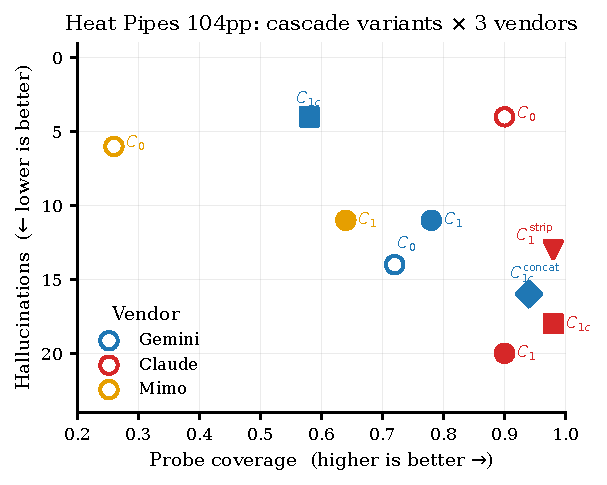
\includegraphics[width=0.55\linewidth]{figures/fig3_heatpipes_pareto.pdf}
\caption{Heat Pipes (104 pages) Pareto frontier across vendors and cascade variants. Gemini cascade is small-Pareto-positive; Claude $C_1$ regresses on faithfulness (4h$\to$20h), leaving $C_0$ on the Pareto frontier (the Mode-B signature); Mimo trades $+5$ halluc for $+38$pp coverage (Modes A+B compounded).}
\label{fig:xvendor_appdx}
\end{figure}

\paragraph{SP-5100 176pp replication.} NASA SP-5100 ``Shock and Vibration Technology'' (1972, 176pp, 47k pdftotext words, 4.00 citation surface forms / 1k words) was chosen as a second long citation-heavy NASA survey for Mode~B replication. Gemini $C_0$ median $46.5$h/0.52 cov $\to C_1$ median $45$h/0.60 cov (range $\{25,45,59\}$ across three judge re-runs of the byte-identical review, i.e.\ judge variance, not Pass-2 variance). Claude $C_1$ median $85$h/0.81 cov (range $\{47,85,85,97\}$ across four judge re-runs, where the originally reported $47$h was a low-end outlier). Mimo $C_1\,60$h/0.23 cov. Claude $C_0$ not realizable: 176 page-images exceed Anthropic's per-request payload limit even with the 1M-context beta. Spot-checking Claude $C_1$ shows the same bibliographic-expansion signature as Heat~Pipes.

\begin{table}[h]
\centering
\small
\caption{\textbf{Within-Claude $C_0$--$C_1$ comparison} on the six NASA papers that fit its multimodal payload (data for Figure~\ref{fig:xmodel}b). Halluc.\ is the GPT-5.4 unsupported-claim count; cov.\ uses the Gemini reference/probes. Hallucinations fall on 5/6 cells; Heat Pipes is the Mode-B exception. Cells are sorted by length.}
\label{tab:claude_within}
\begin{tabular}{lrrrrr}
\toprule
Cell & len & $C_0$ h/cov & $C_1$ h/cov & $\Delta_h$ & $\Delta_{\rm cov}$ \\
\midrule
Wagging Tail      &   9p & 5 / 0.959  & 2 / 0.980  & $-3$  & $+0.021$ \\
Env Test          &  18p & 3 / 1.000  & 2 / 1.000  & $-1$  & $\pm0.000$ \\
Dynamic Response  &  41p & 2 / 1.000  & 1 / 0.960  & $-1$  & $-0.040$ \\
Natural Vibration &  42p & 5 / 0.915  & 4 / 0.851  & $-1$  & $-0.064$ \\
Thermal Analysis  &  66p & 11 / 0.920 & \textbf{4 / 1.000} & $-7$ & $+0.080$ \\
Heat Pipes        & 104p & \textbf{4} / 0.900 & 20 / 0.900 & $+16$ & $\pm0.000$ \\
\midrule
\multicolumn{4}{l}{\emph{direction (noise floor $|\Delta_h|{\ge}1$, $|\Delta_{\rm cov}|{\ge}0.04$)}} & 5/6 $\downarrow$ & --- \\
\bottomrule
\end{tabular}
\end{table}

\paragraph{Modern arXiv reviews.} Gemini Fairness~AI: $14$h/0.50 $\to$ $15$h/0.40 ($-10$pp coverage, Mode~A). Claude $C_1\,23$h/0.70, and Mimo $C_1\,18$h/0.32. Gemini Megagauss: $C_0$ median $36$h/0.66 $\to C_1$ median $30$h/0.68 (high baseline-halluc physics review). Claude $C_1\,17$h/0.92, and Mimo $C_1\,19$h/0.26. Gemini Perovskite: $2$h/0.90 $\to$ $3$h/0.74 at $n{=}1$ ($-6$pp under multi-seed, near-noise-floor). Claude $C_1\,0$h/0.90, and Mimo $C_1\,2$h/0.90. The arXiv pattern (Mode~A on $2/3$) is opposite-direction from the NASA pattern despite comparable page counts. We attribute this to (a)~arXiv full-color 200~DPI rendering carrying more visual signal per page, and (b)~higher typesetting density forcing more aggressive $C_1$ compression at the same output budget.

\section{Mixed-model audio cascade: decomposition unlocks text-only models}
\label{appdx:mixed}

The same-weights audio cascade is Gemini-only by API constraint (\S\ref{sec:discussion}). In production one would not use one model for everything; one would use the best model per stage. This probe does exactly that, and is therefore \emph{off-protocol}: it mixes vendors across stages, so it speaks to the generality of \emph{decomposition}, not the same-weights claim. We take an \emph{independent}, non-Google Pass-1 transcript from OpenAI \texttt{gpt-audio} (chunked, full quality---distinct from the Gemini reference used for judging), then run a text-only synthesis Pass-2 with three frontier text models, two of which (Claude Opus 4.7, GPT-5.4) cannot ingest audio at all on their own. Reviews are scored on the shared Pro reference and probes with the GPT-5.4 judge, plus a Claude-judge cross-check on the GPT-5.4-authored review to rule out self-grading.

The result is unambiguous (Table~\ref{tab:mixed}; Figure~\ref{fig:xmodel}d): on all three cells, every mixed pipeline beats Gemini's \emph{end-to-end} $C_0$ on both axes---coverage rises to $0.85$--$1.00$ (vs $C_0$ $0.63$--$0.88$) and hallucinations fall to $2$--$9$ (vs $11$--$17$). Decomposition thus \emph{unlocks} text-only frontier models for audio review and lets them outperform the native audio model's end-to-end pass, using an off-the-shelf transcript. The GPT-5.4 self-grading concern is unfounded: the Claude judge scores the GPT-5.4-authored reviews \emph{lower} on hallucinations (1/3/3 vs the GPT-5.4 judge's 3/6/9), consistent with the $0.71\times$ inter-judge ratio (\S\ref{sec:robust}). Where the mixed pipeline trails the Gemini same-weights $C_1$ (most clearly on MIT: coverage $0.85$--$0.90$ vs $0.98$ across all three Pass-2 models), the deficit tracks \texttt{gpt-audio}'s lossier transcript, i.e.\ the ceiling is set by Pass-1 transcript quality, exactly as the perceive--externalize--synthesize account predicts.

\begin{table}[h]
\centering
\small
\caption{Mixed-model audio cascade (off-protocol): independent \texttt{gpt-audio} Pass-1 transcript $\to$ text-only Pass-2 by each model, vs Gemini~3.1~Pro end-to-end $C_0$. Hallucinations\,h / probe-coverage, GPT-5.4 judge; the parenthetical on GPT-5.4 is the Claude-judge cross-check. Claude and GPT-5.4 take no audio input, so their only route to an audio review is via the cascade---and it beats Gemini's $C_0$ on every cell.}
\label{tab:mixed}
\setlength{\tabcolsep}{3pt}
\begin{tabular}{lcccc}
\toprule
Cell & Gemini $C_0$ (e2e) & \texttt{gpt-audio}$\to$Claude & \texttt{gpt-audio}$\to$GPT-5.4 & \texttt{gpt-audio}$\to$Gemini \\
\midrule
3B1B Attention & 11h / 0.88 & \textbf{2h / 1.00} & 3h / 1.00 \,(1h / 1.00) & 5h / 1.00 \\
Karpathy       & 13h / 0.63 & 6h / 0.98 & 6h / 1.00 \,(3h / 1.00) & 5h / 0.90 \\
MIT 6.034      & 17h / 0.77 & 3h / 0.90 & 9h / 0.90 \,(3h / 0.92) & 5h / 0.85 \\
\bottomrule
\end{tabular}
\end{table}

\section{Cross-model audio: Gemini 2.5 Flash (clean, no bitrate confound)}
\label{appdx:flash_audio}

Table~\ref{tab:flash_audio} reports a full-quality $C_0$-vs-$C_1$ comparison with Gemini~2.5~Flash as the subject model (same reused Pro reference and probes, same GPT-5.4 judge), over five representative audio cells; Figure~\ref{fig:xmodel}c plots it against the Pro arm. Unlike the Mimo audio arm, the audio is the full 32~kbps source (no OpenRouter 10MB cap), so there is no audio-quality confound. 2.5~Flash is a strong end-to-end audio reader: its $C_0$ coverage exceeds Gemini~3.1~Pro's on all five cells (only on Harvard does it pay for that coverage with more hallucinations, 19 vs Pro's 11), leaving little headroom. The cascade direction then follows the inverse-baseline law---a clear win on the two headroom cells (MIT, Harvard), flat on the saturated NeurIPS panel, and a faithfulness regression on Karpathy (where $C_0$ is already $0.92$/3h). Net: faithfulness improves on 3/5 and coverage on 1/5, a smaller and headroom-gated effect rather than the uniform audio win seen on Pro. Gemini~3~Flash was attempted as a second subject but its verbatim Pass-1 transcription returns empty under the model's recitation filter on copyrighted audio, so the cascade is not realizable on it.

\begin{table}[h]
\centering
\small
\caption{Gemini 2.5 Flash audio $C_0$-vs-$C_1$ (five cells, full-quality audio, GPT-5.4 judge on the reused Pro reference/probes). Sorted by length. The win tracks $C_0$ headroom: large where $C_0$ is weak (MIT, Harvard), absent where $C_0$ is already strong (NeurIPS, Karpathy).}
\label{tab:flash_audio}
\begin{tabular}{lrrrrr}
\toprule
Cell & min & $C_0$ h/cov & $C_1$ h/cov & $\Delta_h$ & $\Delta_{\rm cov}$ \\
\midrule
3B1B Attention & 26 & 5 / 0.900  & 1 / 0.920  & $-4$ & $+0.020$ \\
NeurIPS panel  & 31 & 5 / 0.980  & 6 / 0.959  & $+1$ & $-0.020$ \\
Karpathy       & 42 & 3 / 0.922  & 9 / 0.902  & $+6$ & $-0.020$ \\
MIT 6.034      & 47 & 7 / 0.833  & \textbf{4 / 0.958} & $-3$ & $+0.125$ \\
Harvard Moot   & 82 & 19 / 0.600 & \textbf{12 / 0.620} & $-7$ & $+0.020$ \\
\bottomrule
\end{tabular}
\end{table}

\section{Iterative refinement ($C_{1\rm iter}$): full results}
\label{appdx:iter}

The three-step pipeline and the high-level verdict are in \S\ref{sec:failure_modes}; Figure~\ref{fig:failure_modes}b plots the per-cell movement and Table~\ref{tab:iter_results} gives the $n{=}5$ numbers.

\begin{table}[h]
\centering
\small
\caption{Iterative refinement ($C_{1\rm iter}$) on seven cells at $n{=}5$, $T{=}0.7$. Hallucinations are mean$\pm$sd and coverage is mean; $\Delta$ is versus a plain $C_1$ baseline re-measured at $n{=}5$. ``Pareto'' improves both axes beyond noise; ``Trade'' exchanges them; ``Net-neg'' loses coverage without a faithfulness gain.}
\label{tab:iter_results}
\begin{tabular}{lrrrrl}
\toprule
Cell (vendor) & $C_1$ baseline & $C_{1\rm iter}$ & $\Delta_{\rm halluc}$ & $\Delta_{\rm cov}$ & Verdict \\
\midrule
Natural Vibration (Gemini) & $7.8{\pm}2.2$ / $0.54$  & $\mathbf{3.6{\pm}1.4}$ / $\mathbf{0.66}$ & $-4.2$  & $+0.13$ & \textbf{Pareto} \\
Heat Pipes (Gemini)        & $14.4{\pm}2.6$ / $0.63$ & $10.6{\pm}3.1$ / $0.46$ & $-3.8$  & $-0.17$ & trade   \\
Heat Pipes (Claude)        & $14.8{\pm}3.5$ / $0.93$ & $14.2{\pm}4.4$ / $0.74$ & $-0.6$  & $-0.20$ & net-neg \\
arXiv Fairness AI (Gemini) & $15.6{\pm}6.6$ / $0.36$ & $21.8{\pm}1.0$ / $0.36$ & $+6.2$  & $+0.01$ & net-neg \\
arXiv Fairness AI (Claude) & $21.0{\pm}3.9$ / $0.58$ & $21.8{\pm}3.2$ / $0.40$ & $+0.8$  & $-0.17$ & net-neg \\
SP-5100 (Claude)           & $62.8{\pm}23$ / $0.74$  & $49.8{\pm}13$ / $0.56$ & $-13.0$ & $-0.18$ & trade   \\
arXiv Megagauss (Claude)   & $40.6{\pm}4.6$ / $0.90$ & $32.2{\pm}8.5$ / $0.64$ & $-8.4$  & $-0.25$ & trade   \\
\bottomrule
\end{tabular}
\end{table}

$C_{1\rm iter}$ targets Mode~B (a verbatim-quote requirement rules out unsupported expansions) but does not relieve Mode~A: the rewrite step itself compresses, so coverage falls on every long cell, and the net verdict is the balance of recovered faithfulness against that compression cost. Two single-seed verdicts did not survive $n{=}5$: the Heat~Pipes~Claude Mode-B ``fix'' (now within noise) and an apparent ``hallucinations increase'' on SP-5100/Megagauss (both counts in fact \emph{fall} at $n{=}5$; the single-seed rises were high-variance GPT-5.4 judge draws on 40--90-claim lists).

\section{Engineering interventions: chunked Pass-2 and citation stripping}
\label{appdx:fixes}

\begin{table}[h]
\centering
\caption{Heat~Pipes Claude 104pp variants. Strip dominates plain $C_1$ at $n{=}1$ on both axes. Chunked combinations do not improve over strip alone. \emph{At $n{=}5$ multi-seed, the strip effect on $C_1$ hallucinations is statistically null} ($\hat\Delta=-1.8\pm2.6$, 95\% CI $[-6.9,+3.3]$).}
\label{tab:hp_claude_variants}
\small
\begin{tabular}{lrrr}
\toprule
Variant & Halluc. & Coverage & Words \\
\midrule
$C_0$ (image baseline) & \textbf{4}  & 0.900 & 3{,}308 \\
$C_1$ (single Pass-2) & 20 & 0.900 & 2{,}077 \\
$C_1^{\rm strip}$ (citations $\to$ \texttt{[REF]}) & \textbf{13} & \textbf{0.980} & 2{,}471 \\
$C_{1c}$ (chunked + merge) & 18 & 0.980 & 2{,}769 \\
$C_{1c}^{\rm concat}$ (chunked, no merge) & 20 & 0.940 & 2{,}777 \\
$C_{1c}^{\rm strip}$ (strip + chunked + merge) & 18 & 0.980 & 2{,}673 \\
$C_{1c}^{\rm strip+concat}$ (strip + chunked, no merge) & 16 & 0.980 & 2{,}766 \\
\bottomrule
\end{tabular}
\end{table}

\paragraph{Mode-B fix replication on 3 new long Claude cells.}
Table~\ref{tab:mode_b_strip_replication} reports the strip intervention across four Claude cells. On SP-5100, the published single-call snapshot $C_1\,47h \to C_1^{\rm strip}\,24h$ initially looked like a clean halving, but the unstripped $C_1$ review judged four times yields $\{47, 85, 85, 97\}$ (median $85$), so the $-23$h effect compares one strip call against a low-end outlier of the unstripped distribution. On Megagauss, strip has essentially no effect ($17\to 19$h, $0.92\to 0.94$ cov). On Fairness~AI only 1 surface form matched our regexes (its citations are author--year, which the numeric-form patterns do not match, so the intervention never touched the text it targets), and the ``stripped'' Pass-2 produced a substantially different review ($23\to 41$h, $0.70\to 0.62$ cov), revealing that Claude's text-only Pass-2 is itself non-deterministic. \textbf{Net Mode-B-fix status: zero replicated cells} (Heat~Pipes retracted at $n{=}5$, Megagauss null, Fairness~AI null-by-design, SP-5100 single-call-each).

\begin{table}[h]
\centering
\caption{Mode~B citation-strip intervention across four long Claude cells. ``surface forms'' = regex hits replaced with \texttt{[REF]}.}
\label{tab:mode_b_strip_replication}
\small
\begin{tabular}{lrrrrrr}
\toprule
Cell & len & surface forms & $C_1$ h & $C_1$ cov & $C_1^{\rm strip}$ h & $C_1^{\rm strip}$ cov \\
\midrule
Heat~Pipes (recall)        & 104p & 55  & 20 & 0.900 & \textbf{13} & \textbf{0.980} \\
SP-5100 (new)              & 176p & 193 & 47 & 0.812 & \textbf{24} & 0.708 \\
arXiv Megagauss (new)      &  75p & 298 & 17 & 0.920 & 19 & 0.940 \\
arXiv Fairness~AI (new)    &  53p & 1   & 23 & 0.700 & 41 & 0.620 \\
\bottomrule
\end{tabular}
\end{table}

\paragraph{Mode-A chunked Pass-2 replication and multi-seed verification.}
$n{=}1$ ($T{=}0$) results are consistent across four papers (Table~\ref{tab:mode_a_chunked_replication}): $C_{1c}^{\rm concat}$ (chunked, no merge) recovers coverage on long sources at a hallucination cost, while $C_{1c}$ (chunked + merge) over-compresses: on Perovskite and Megagauss the merge variant collapses to $0.10$ and $0.12$ coverage respectively. At $n{=}5$ multi-seed (Table~\ref{tab:chunked_multiseed_appdx}), the chunked-Pass-2 direction survives on Fairness~AI and Perovskite but \emph{not} on Megagauss, whose original $n{=}1$ ($0.74$cov) sits above the entire $n{=}5$ envelope $[0.64, 0.68]$ at $T{=}0.7$. We retract the original ``chunked Pass-2 lifts coverage on all three arXiv counter-cells'' claim.

\begin{table}[h]
\centering
\caption{Chunked-Pass-2 ($n{=}1$, $T{=}0$) across four Gemini long-paper cells.}
\label{tab:mode_a_chunked_replication}
\small
\begin{tabular}{lrrrrr}
\toprule
Cell & len & $C_1$ h/cov & $C_{1c}$ h/cov & $C_{1c}^{\rm concat}$ h/cov & $\Delta_{\rm cov}^{\rm concat}$ \\
\midrule
Heat~Pipes (recall)    & 104p & 11 / 0.78 & 4 / 0.58 & 16 / 0.94 & $+0.16$ \\
arXiv Perovskite (new) &  80p & 3  / 0.74 & 1 / 0.10 & 13 / 0.82 & $+0.08$ \\
arXiv Megagauss (new)  &  75p & 32 / 0.68 & 0 / 0.12 & 36 / 0.74 & $+0.06$ \\
arXiv Fairness~AI (new)&  53p & 15 / 0.40 & 5 / 0.32 & 37 / 0.52 & $+0.12$ \\
\bottomrule
\end{tabular}
\end{table}

\begin{table}[h]
\centering
\small
\caption{Multi-seed verification of $C_{1c}^{\rm concat}$ on the three arXiv cells ($n{=}5$ seeds, Gemini~3.1~Pro Pass-2, $T{=}0.7$).}
\label{tab:chunked_multiseed_appdx}
\resizebox{\textwidth}{!}{%
\begin{tabular}{lrrrrrl}
\toprule
Cell & $C_1$ baseline & orig $n{=}1$ & $n{=}5$ halluc & $n{=}5$ cov & cov range & dir.\ survives \\
\midrule
arXiv Fairness AI & 15h / 0.40 & 37h / 0.52 & $31.6\pm1.9$ & $0.496\pm0.055$ & $[0.440, 0.580]$ & yes \\
arXiv Megagauss   & 32h / 0.68 & 36h / 0.74 & $42.2\pm4.3$ & $0.664\pm0.017$ & $[0.640, 0.680]$ & \textbf{NO} \\
arXiv Perovskite  & 3h / 0.74  & 13h / 0.82 & $16.6\pm2.5$ & $0.832\pm0.033$ & $[0.800, 0.880]$ & yes \\
\bottomrule
\end{tabular}%
}
\end{table}

\paragraph{Citation stripping on Gemini Natural Vibration ($n{=}5$ verified).}
At $n{=}1$ ($T{=}0$), strip moves halluc $5\to 12$ but coverage $0.49\to 0.81$ ($+32$pp). At $n{=}5$ ($T{=}0.7$, seeds $1$--$5$): halluc $\{15,11,9,8,8\}$ with mean $10.2$, and coverage $\{0.660, 0.723, 0.702, 0.511, 0.766\}$ with mean $0.672$. The strip-vs-$C_1$ direction (cov gain at halluc cost) survives all 5 seeds. The magnitude on coverage is $+18$pp (mean) versus the original $+32$pp single-seed reading.

\section{Multi-seed envelopes on the four headline cells}
\label{appdx:multiseed}

Figure~\ref{fig:robustness}b (main text) plots the envelopes; Table~\ref{tab:headline_multiseed_appdx} gives the numbers.

\begin{table}[h]
\centering
\small
\caption{Per-cell multi-seed envelopes for the four headline cells (Gemini $C_1$ Pass-2 at $T{=}0.7$, seeds 1--5). ``base-in-envelope?'' checks whether the $n{=}1$ value sits within the per-seed range.}
\label{tab:headline_multiseed_appdx}
\begin{tabular}{lrrrl}
\toprule
Cell & orig $n{=}1$ & $n{=}5$ halluc & $n{=}5$ cov & base-in-envelope? \\
\midrule
MIT 6.034 Winston   & $4$h / $0.98$ & $7.4 \pm 1.5$ & $0.971 \pm 0.028$ & cov yes; halluc \textbf{NO} (low) \\
Sapolsky Behavioral & $15$h / $0.94$ & $14.5 \pm 2.5$ & $0.898 \pm 0.017$ & halluc yes; cov \textbf{NO} (high) \\
Heat Pipes Gemini   & $11$h / $0.78$ & $15.4 \pm 2.7$ & $0.732 \pm 0.056$ & cov yes; halluc \textbf{NO} (low) \\
arXiv Perovskite    & $3$h / $0.74$ & $4.8 \pm 2.2$ & $0.844 \pm 0.056$ & halluc yes; cov \textbf{NO} (low) \\
\bottomrule
\end{tabular}
\end{table}

Two readings: (1)~the published $T{=}0$ baselines are mostly representative of the $T{=}0.7$ distribution on the headline cells, since every cell's $n{=}5$ envelope overlaps the published number on at least one axis. (2)~Perovskite was the seed-envelope point farthest from the multi-seed mean ($10$pp coverage below it), and under multi-seed verification its cascade-cov loss reads $-6$pp rather than $-16$pp. We retain Perovskite as a near-noise-floor cell and treat its earlier ``Mode-A counter-cell'' label as overstated at $n{=}1$.

\section{Three sources of stochasticity}
\label{appdx:stoch}

\begin{figure}[h]
\centering
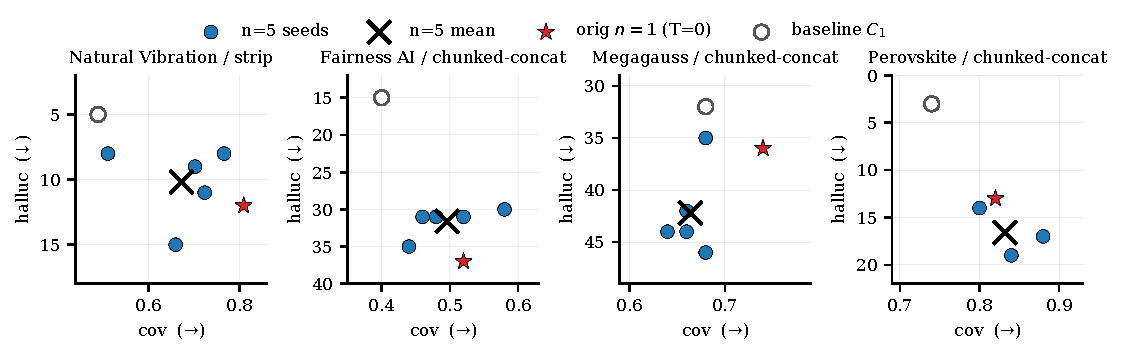
\includegraphics[width=\linewidth]{figures/fig6_multiseed_envelopes.pdf}
\caption{\textbf{$n{=}5$ multi-seed envelopes for four intervention checks.} Blue dots are Pass-2 seeds ($T{=}0.7$), black $\times$ their mean, red stars the original $n{=}1$ result, and open circles plain $C_1$. The original result lies within the envelope for NV strip, Fairness AI, and Perovskite, but not Megagauss; its chunked-Pass-2 coverage claim is therefore retracted.}
\label{fig:multiseed_envelopes_appdx}
\end{figure}


\paragraph{Detailed decomposition.}
\emph{(a)~Claude Pass-2 generation variance.} Same input + same API + same prompt: Heat~Pipes Claude $C_1$ swings $20\to 9$ between two runs (strip $13\to 14$ more stable), and the deltas are large enough that the strip effect cannot be distinguished from Pass-2 noise. Claude Opus 4.7 deprecates the \texttt{temperature} parameter so determinism cannot be enforced from the SDK. \emph{(b)~Gemini Pass-2 generation variance.} At \texttt{temperature=0.0}, two of three Gemini Pass-2 re-runs produced byte-identical output (MD5 match) on Heat~Pipes / SP-5100, and the third differed in similar length (1929 vs 1815 words, $\Delta h = +6$). Gemini is therefore mostly but not strictly deterministic, consistent with GPU-level non-associativity. \emph{(c)~GPT-5.4 high-reasoning judge variance.} Essentially deterministic on low-count cells ($\pm 1$ on Heat~Pipes Claude across three re-judgments) but substantially stochastic on high-count cells ($\pm 25$ on SP-5100, $\pm 17$ on the byte-identical SP-5100 Gemini review). We attribute this to long unsupported-claim lists running up against our 24k-token completion budget, so the judge truncates and resamples across calls. Coverage is stable on every cell across judge re-runs.

\paragraph{$n{=}5$ multi-seed verification on Heat Pipes Claude.} $C_1$ halluc $\{9,11,11,15,20\}$ (mean $13.2$, stdev $4.4$, range 9--20), and $C_1^{\rm strip}$ halluc $\{5,11,13,14,14\}$ (mean $11.4$, stdev $3.8$, range 5--14). Coverage means identical ($0.936$ both) with similar spread. Strip effect on hallucinations at $n{=}5$: $\hat{\Delta}=-1.8$, SE $\approx 2.6$, 95\% CI $[-6.9, +3.3]$, which crosses zero. \textbf{The Mode~B fix is statistically null on Claude/Heat~Pipes at $n{=}5$.}

\begin{table}[h]
\centering
\caption{Stochasticity decomposition. Top: Claude Pass-2 generation variance (different reviews, same prompt, judged once each). Bottom: GPT-5.4 judge variance on the \emph{same} Claude $C_1$ review file (one review, judged multiple times).}
\label{tab:claude_stochasticity_appdx}
\small
\begin{tabular}{lllllr}
\toprule
Cell & Condition & Run 1 & Run 2 & $\Delta h$ & $\Delta \mathrm{cov}$ \\
\midrule
\multicolumn{6}{l}{\emph{Claude Pass-2 generation variance}} \\
Heat Pipes 104p     & $C_1$           & 20h / 0.90 & 9h  / 0.90 & $-11$ & $\pm 0.00$ \\
                    & $C_1^{\rm strip}$ & 13h / 0.98 & 14h / 0.88 & $+1$  & $-0.10$ \\
SP-5100 176p        & $C_1$           & 47h / 0.81 & 79h / 0.81 & $+32$ & $\pm 0.00$ \\
                    & $C_1^{\rm strip}$ & 24h / 0.71 & 97h / 0.77 & $+73$ & $+0.06$ \\
Fairness AI 53p     & $C_1$           & 23h / 0.70 & 27h / 0.66 & $+4$  & $-0.04$ \\
                    & $C_1^{\rm strip}$ & 41h / 0.62 & 17h / 0.60 & $-24$ & $-0.02$ \\
\midrule
\multicolumn{6}{l}{\emph{GPT-5.4 judge variance (same review, judged multiple times)}} \\
Heat Pipes 104p     & $C_1$ (calls 1--3) & 20h / 0.90 & 21h / 0.92 & $+1$ & $+0.02$ \\
SP-5100 176p        & $C_1$ (calls 1--4) & 47h / 0.81 & 97h / 0.81 & $+50$ & $\pm 0.00$ \\
\bottomrule
\end{tabular}
\end{table}

\section{Inter-judge details}
\label{appdx:inter_judge}

Figure~\ref{fig:robustness}a (main text) plots the 22 cell--condition pairs (21 Gemini cells plus the Thermal-Claude cross-vendor cell); the tables below give the per-cell counts on the original 10 cells (per-cell deltas for the remaining cells are released in the repository).

\begin{table}[h]
\centering
\small
\caption{Inter-judge hallucination counts on the original 10 cells. Direction $\checkmark$ means both judges agree on the sign of $C_0\to C_1$. The full 21-cell direction counts are $19/21$ coverage and $14/21$ hallucination (\S\ref{sec:robust}).}
\label{tab:inter_judge_halluc}
\begin{tabular}{lrrrrc}
\toprule
& \multicolumn{2}{c}{GPT-5.4} & \multicolumn{2}{c}{Claude} & Direction \\
\cmidrule(lr){2-3}\cmidrule(lr){4-5}
Cell & $C_0$ & $C_1$ & $C_0$ & $C_1$ & agree? \\
\midrule
Karpathy review            & 13 & 3  & 7  & 4  & \checkmark \\
Karpathy mtg-min           & 4  & 2  & 1  & 0  & \checkmark \\
SNAC mtg-min               & 14 & 11 & 10 & 11 & \texttimes  \\
Wagging Tail (9pp)         & 3  & 1  & 2  & 2  & \texttimes  \\
Env Test (18pp)            & 5  & 4  & 0  & 2  & \texttimes  \\
Dynamic Response (41pp)    & 3  & 2  & 1  & 0  & \checkmark \\
Natural Vibration (42pp)   & 4  & 5  & 2  & 4  & \checkmark \\
Thermal Analysis (66pp)    & 5  & 2  & 2  & 1  & \checkmark \\
Heat Pipes (104pp)         & 14 & 11 & 12 & 11 & \checkmark \\
Thermal Analysis Claude    & 11 & 4  & 9  & 4  & \checkmark \\
\bottomrule
\end{tabular}
\end{table}

\begin{table}[h]
\centering
\small
\caption{Inter-judge probe-coverage counts (probes covered out of $n$) on the original 10 cells.}
\label{tab:inter_judge_cov}
\begin{tabular}{lrrrrrc}
\toprule
& & \multicolumn{2}{c}{GPT-5.4} & \multicolumn{2}{c}{Claude} & Direction \\
\cmidrule(lr){3-4}\cmidrule(lr){5-6}
Cell & $n$ & $C_0$ & $C_1$ & $C_0$ & $C_1$ & agree? \\
\midrule
Karpathy review            & 51 & 32 & 49 & 38 & 49 & \checkmark \\
Karpathy mtg-min           & 50 & 8  & 17 & 13 & 21 & \checkmark \\
SNAC mtg-min               & 49 & 14 & 26 & 15 & 28 & \checkmark \\
Wagging Tail (9pp)         & 49 & 39 & 38 & 40 & 38 & \checkmark \\
Env Test (18pp)            & 50 & 44 & 46 & 46 & 49 & \checkmark \\
Dynamic Response (41pp)    & 50 & 29 & 35 & 32 & 36 & \checkmark \\
Natural Vibration (42pp)   & 47 & 31 & 23 & 32 & 28 & \checkmark \\
Thermal Analysis (66pp)    & 50 & 34 & 42 & 34 & 45 & \checkmark \\
Heat Pipes (104pp)         & 50 & 36 & 39 & 39 & 41 & \checkmark \\
Thermal Analysis Claude    & 50 & 46 & 50 & 46 & 49 & \checkmark \\
\bottomrule
\end{tabular}
\end{table}

Per-probe agreement (the fraction of probes the two judges classify identically as COVERED / MISSING) ranges $0.882$--$1.000$ across the (cell, condition) pairs, median $\approx 0.94$. Two of the three hallucination-direction disagreements on the original 10 cells (Wagging~Tail, Env~Test) are near-tie cells with $\le 5$ hallucinations under both judges. The third (SNAC) is driven by the judges assigning different $C_0$ baselines (14 vs 10) while agreeing on $C_1$.

\section{Probe-circularity and reference-bias check tables}
\label{appdx:probe_circ}

Figure~\ref{fig:robustness}c,d (main text) plots both checks; the tables below give the numbers.

\begin{table}[h]
\centering
\small
\caption{Probe-circularity check on 7 cells spanning the cascade-direction spectrum. ``Original'' = published numbers (GPT-5.4-extracted probes, GPT-5.4 judge); the other columns re-extract probes via Claude and score under each judge.}
\label{tab:probe_circularity_appdx}
\begin{tabular}{lrrr}
\toprule
Cell (orig $\to$ Claude-extracted probes) & $\Delta_{\rm cov}$ (orig) & Claude-pr.\ / GPT & Claude-pr.\ / Claude \\
\midrule
Karpathy review (51 $\to$ 55) [audio]     & $+0.333$ & $+0.400$ & $+0.236$ \\
MIT 6.034 (48 $\to$ 50) [audio]            & $+0.208$ & $+0.180$ & $+0.120$ \\
Heat Pipes 104pp (50 $\to$ 60) [paper]     & $+0.060$ & $+0.050$ & $+0.033$ \\
Natural Vibration 42pp (47 $\to$ 50) [paper] & $-0.170$ & $-0.160$ & $-0.200$ \\
arXiv Fairness AI 53pp (50 $\to$ 50) [paper] & $-0.100$ & $-0.100$ & $+0.040$ \\
arXiv Megagauss 75pp (50 $\to$ 60) [paper]   & $+0.020$ & $+0.000$ & $+0.000$ \\
arXiv Perovskite 80pp (50 $\to$ 54) [paper]  & $-0.160$ & $-0.167$ & $-0.111$ \\
\bottomrule
\end{tabular}
\end{table}

\begin{table}[h]
\centering
\small
\caption{Reference-bias check on 4 cells. The non-Gemini reference rows replace OCR/ASR only, and probes are re-extracted by Claude. ``orig'' = Gemini reference + GPT-5.4 probes + GPT-5.4 judge.}
\label{tab:ref_bias_appdx}
\begin{tabular}{lcrrrr}
\toprule
Cell & Reference & $\Delta_h$ orig & $\Delta_h$ alt & $\Delta_{\rm cov}$ orig & $\Delta_{\rm cov}$ alt \\
\midrule
3B1B Attention 26m   & Whisper-base / GPT-5.4 & $-11$ & $-7$ & $+0.080$ & $+0.120$ \\
3B1B Attention 26m   & Whisper-base / Claude  & $-11$ & $-6$ & $+0.080$ & $+0.060$ \\
Karpathy review 42m  & Whisper-base / GPT-5.4 & $-10$ & $-4$ & $+0.333$ & $+0.353$ \\
Karpathy review 42m  & Whisper-base / Claude  & $-10$ & $-6$ & $+0.333$ & $+0.176$ \\
Wagging Tail 9p      & EasyOCR / GPT-5.4      & $-2$  & $-1$ & $-0.020$ & $-0.019$ \\
Wagging Tail 9p      & EasyOCR / Claude       & $-2$  & $-3$ & $-0.020$ & $-0.038$ \\
Thermal Analysis 66p & EasyOCR / GPT-5.4      & $-3$  & $\mathbf{+2}$ & $+0.160$ & $+0.094$ \\
Thermal Analysis 66p & EasyOCR / Claude       & $-3$  & $\mathbf{+1}$ & $+0.160$ & $+0.094$ \\
\bottomrule
\end{tabular}
\end{table}

The Thermal hallucination-direction flip under EasyOCR is a reference-side artifact: EasyOCR's transcript is $\approx 21\%$ shorter and loses figure captions, so claims the cascade correctly reproduces read as unsupported against the noisier reference.

\section{Per-cell hallucinations per 1k output words}
\label{appdx:perword}

\begin{table}[h]
\centering
\small
\caption{Hallucination density (per 1k output words) on Thermal Analysis (66 pages).}
\label{tab:per_word_halluc}
\begin{tabular}{lrr}
\toprule
& $C_0$ & $C_1$ \\
\midrule
Gemini 3.1 Pro  & 4.2 & \textbf{1.4} \\
Claude Opus 4.7 & 3.7 & \textbf{1.4} \\
Mimo v2-omni    & 4.9 & 5.4 \\
\bottomrule
\end{tabular}
\end{table}

End-to-end hallucination rates differ per vendor (3.7 / 4.2 / 4.9 per 1k), and cascade brings Gemini and Claude to a common $\approx 1.4$ per 1k floor on the moderate-length paper. Mimo does not converge to this floor.

\begin{table}[h]
\centering
\small
\caption{Hallucination density (per 1k output words) on Heat Pipes (104pp). Claude $C_1$ reaches 9.6/1k, versus 1.4/1k on Thermal, consistent with Mode~B rather than a general verbosity effect.}
\label{tab:per_word_halluc_hp}
\begin{tabular}{lrr}
\toprule
& $C_0$ & $C_1$ \\
\midrule
Gemini 3.1 Pro                            & 7.6 & 6.1 \\
Claude Opus 4.7                           & \textbf{1.2} & \textbf{9.6} \\
Claude Opus 4.7 ($C_1^{\rm strip}$)       & --- & 5.3 \\
Mimo v2-omni                              & 7.0 & 6.9 \\
\bottomrule
\end{tabular}
\end{table}

Claude's per-1k hallucination rate jumps from 1.2 ($C_0$) to 9.6 ($C_1$) on Heat~Pipes, an $8\times$ increase that survives length normalization. The same model on the same protocol on Thermal~66pp moved 3.7$\to$1.4. Citation stripping pulls Heat~Pipes Claude back to 5.3/1k. Gemini and Mimo on the same paper sit at $6$--$8$/1k regardless of cascade variant, indicating that the 1.4/1k floor reached on Thermal is not a property of the cascade in general, but of the specific (model, source) interaction.

\section{Specific hallucination examples (Heat Pipes Claude)}
\label{appdx:examples}

The 20 unsupported claims from Claude $C_1$ on Heat~Pipes 104pp are dominated by training-prior expansions of bibliographic abbreviations:

\begin{itemize}
\itemsep0pt
\item ``Cotter's 1965 analysis (LA-3246-MS)'': the transcript cites only ``Reference 2 (Cotter)'', so the year and report number are training-data details.
\item ``correlation from Allingham and McEntire (1961)'': the transcript only says ``Ref.~12'', so the author names and year are training-data details.
\item ``McAdams' laminar horizontal-tube formula'': the transcript says ``Reference 13 for laminar condensation on horizontal tubes'', so ``McAdams'' is a training-data detail.
\item ``Vapor chamber-fin radiator (Haller, Lieblein, and Lindow at NASA Lewis)'': the transcript says only ``proposed by Haller, et al of NASA''.
\end{itemize}

One outright misreading: the transcript states the no-boiling condition as $p_v - p_\ell \le 2\sigma\cos\theta/r_c$, but Claude's review writes $\ge$. This is a sign error in Pass-2 reading of Pass-1 text, not training-prior leak.

\section{Code and data availability}
\label{sec:code}
\label{appdx:code}

\begin{sloppypar}
All code, prompts, per-cell judgments, and the mechanistic-experiment artifacts (including the frontier modality probes, the running-example run directory, and the within-Claude cross-vendor comparison) are released in the project repository, whose README documents the pipelines and the exact commands to reproduce every cell, table, and figure in this paper.
\end{sloppypar}

\end{document}
